% !chktex-file 8
% !chktex-file 1

% Document type
\documentclass[french,twoside]{article}
\usepackage{edify}

\usetikzlibrary{automata}
\usetikzlibrary{arrows}
\usetikzlibrary{positioning}

\title{Complexité en état d'opération sur des langages rationnels}
\date{\today}
\author{
  Edouard
  % LTeX: enabled=false
  HADDAG
  % LTeX: enabled=true
}
% LTeX: enabled=false
\logo{logo-univ-rouen-normandie-noir.png}
% LTeX: enabled=true
\headerrf{Université de Rouen Normandie}
\headerrs{Application Informatique}
\abs{
  Dans cet article, nous étudions deux transformations particulières de
  langages rationnels~: le << trognon >> et le << langage permuté >>. Nous
  définissons formellement ces deux constructions et proposons pour chacune un
  algorithme permettant de calculer un automate non déterministe reconnaissant
  le langage transformé. Nous démontrons la correction de ces algorithmes et
  analysons leur complexité en nombre d’états dans le pire des cas.
}

\begin{document}

\maketitle

\newpage

\tableofcontents

% !chktex-file 8

\subsection{Présentation du papier}

\setframetitle{Présentation du papier}

\begin{frame}{\myframetitle}
  \begin{block}{Présentation du papier}
    % LTex: language=en
    \textit{State complexity of some operations on binary regular
    languages}\footnotemark{}
    % LTex: language=fr

    \vphantom{}

    Par \textbf{Galina Jirásková}, publié dans
    % LTex: language=en
    \textit{\underline{Theoretical Computer Science, 330.2}}
    % LTex: language=fr%
    en 2005
  \end{block}
  \footnotetext{\hyperlink{JIRASKOVA2005287}{\cite{JIRASKOVA2005287}}}
\end{frame}

\section{Introduction}

\subsection{Prémisse}

\subsubsection{Alphabet et Mot}

\setframetitle{Alphabet et Mot}

\begin{frame}{\myframetitle}
  \begin{definition}[Alphabet]
    Un << alphabet >> \(\Sigma\) est un ensemble fini non-vide de symboles.
  \end{definition}

  \pause[]

  \begin{definition}[Mot]
    Un << mot >> \(w\) est une suite finie de symboles sur un alphabet
    \(\Sigma\). La suite vide de symbole sera notée par \(\varepsilon\).
  \end{definition}

  \pause[]

  \begin{example}
    \centering
    \vspace{-1.5\topsep}
    \begin{gather*}
      \Sigma = \{a, b\} \\
      w = abba
    \end{gather*}
  \end{example}
\end{frame}

\begin{frame}{\myframetitle}
  \begin{definition}[Concaténation d'un mot]
    L'opération \(\cdot\) désigne la << concaténation >> de deux mots.
  \end{definition}

  \pause[]

  \begin{example}
    \centering
    \vspace{-1.5\topsep}
    \begin{gather*}
      u = aa \text{ et } v = bb \\
      w = u \cdot v = aabb
    \end{gather*}
  \end{example}
\end{frame}

\begin{frame}{\myframetitle}
  \begin{definition}[Le miroir d'un mot]
    On notera \(\overleftarrow w\), le << miroir >> du mot \(w\).
  \end{definition}

  \pause[]

  \begin{example}
    \vspace{-1.5\topsep}
    \begin{align*}
      u &= abcd\\
      \overleftarrow u &= dcba
    \end{align*}
  \end{example}
\end{frame}

\subsubsection{Langage}

\setframetitle{Langage}

\begin{frame}{\myframetitle}
  \begin{definition}[Langage]
    Un << langage >> \(L\) est un ensemble de mots sur un alphabet \(\Sigma\).
  \end{definition}

  \pause[]

  \begin{example}
    \vspace{-1.5\topsep}
    \begin{gather*}
      L = \{\varepsilon, aa, bb, abab\}
    \end{gather*}
  \end{example}
\end{frame}

\begin{frame}{\myframetitle}
  \begin{definition}[La concaténation]
    La << concaténation >> est définie grâce à la concaténation des mots~:

    \begin{alignat*}{2}
      &L_1 &&= \{a, b\} \\
      &L_2 &&= \{c, d\} \\
      &L_1 \cdot L_2 &&= \{ac, ad, bc, bd\} \\
    \end{alignat*}
  \end{definition}
\end{frame}

\begin{frame}{\myframetitle}
  \begin{definition}[La copie n-ième]
    On définit la << copie n-ième >> d'un langage \(L\) noté \(L^n\)~:

    \begin{alignat*}{2}
      &L_1 &&= \{a, b\} \\
      &L_1^2 &&= \{aa, ab, bb, ba\}
    \end{alignat*}
  \end{definition}
\end{frame}

\begin{frame}{\myframetitle}
  \begin{definition}[L'étoile (de \textit{Kleene}) d'un langage]
    On peut définir << l'étoile >> d'un langage notée \(L^*\)~:
    % LTeX: enabled=false
    \begin{align*}
      L^* = \bigcup_{i \geq 0} L^i
    \end{align*}
    % LTeX: enabled=true
  \end{definition}

  \pause[]

  \begin{example}
    \vspace{-1.5\topsep}
    \begin{align*}
      &L = \{a, b\} \\
      &L^* = \{\varepsilon, a, b, aa, ab, \ldots\}
    \end{align*}
  \end{example}
\end{frame}

\begin{frame}{\myframetitle}
  \begin{definition}[Le langage de l'ensemble des mots]
    L'ensemble des mots possible sur l'alphabet \(\Sigma\) sera noté
    \(\Sigma^*\).
  \end{definition}

  \pause[]

  \begin{definition}[Le langage miroir]
    On pourra noter \(\overleftarrow L\), << le langage miroir >> de \(L\), qui
    sera le langage des miroirs des mots de \(L\)~:
    \begin{align*}
      \overleftarrow L = \{\overleftarrow w ~|~ w \in L\}
    \end{align*}
  \end{definition}

  \pause[]

  \begin{block}{Autres opérations}
    Les langages étant des ensembles, leurs opérations peuvent être étendues
    aux langages.
  \end{block}
\end{frame}

\begin{frame}{\myframetitle}
  \begin{definition}[Les langages rationnels]
    L'ensemble des << langages rationnels >> sur \(\Sigma\), noté
    \(\RAT(\Sigma^*)\), est le plus petit ensemble de langages sur \(\Sigma\)
    qui vérifie~:

    \vphantom{}

    \begin{itemize}
      \item \(\RAT(\Sigma^*)\) contient \(\varnothing\) et \(\{a\}\) avec \(a
        \in \Sigma\).
      \item \(\RAT(\Sigma^*)\) est fermé pour l'union, la concaténation et
        l'étoile.
    \end{itemize}
  \end{definition}
\end{frame}

\subsubsection{Automate}

\setframetitle{Automate}

\begin{frame}{\myframetitle}
  \begin{definition}[Automate]
    \(M = (Q, I, F, \delta)\) avec \(Q = \{q_1, q_2, q_3\}\), \(I = \{q_1\}\) et
    \(F = \{q_3\}\).
    \begin{center}
      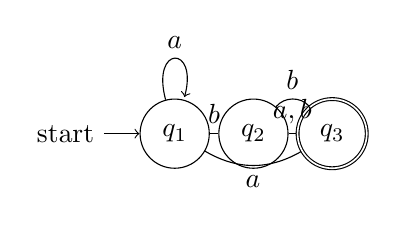
\begin{tikzpicture}
        \node[state, initial] (q1) {\(q_1\)};
        \node[state, right of=q1] (q2) {\(q_2\)};
        \node[state, accepting, right of=q2] (q3) {\(q_3\)};

        \draw
        (q1) edge[loop above] node{\(a\)} (q1)
        (q1) edge[above] node{\(b\)} (q2)
        (q1) edge[bend right, below] node{\(a\)} (q3)
        (q2) edge[above] node{\(a,b\)} (q3)
        (q3) edge[bend right=50, above] node{\(b\)} (q2);
      \end{tikzpicture}
    \end{center}
  \end{definition}
\end{frame}

\begin{frame}{\myframetitle}
  \begin{definition}[L'acceptation d'un mot]
    Le mot \(aba\) est << accepté >>~:
    \begin{center}
      \begin{tikzpicture}
        \node[state, initial] (q1) {\(q_1\)};
        \node[state, right of=q1] (q2) {\(q_2\)};
        \node[state, accepting, right of=q2] (q3) {\(q_3\)};

        \only<1> {\draw (q1) edge[loop above] node{\(a\)} (q1);}
        \only<1-2> {\draw (q1) edge[above] node{\(b\)} (q2);}
        \only<1-3> {\draw (q2) edge[above] node{\(a,b\)} (q3);}

        \only<2-> {\draw (q1) edge[loop above, red] node{\(a\)} (q1);}
        \only<3-> {\draw (q1) edge[above, red] node{\(b\)} (q2);}
        \only<4-> {\draw (q2) edge[above, red] node{\(a,b\)} (q3);}

        \draw
        (q3) edge[bend right=50, above] node{\(b\)} (q2)
        (q1) edge[bend right, below] node{\(a\)} (q3);
      \end{tikzpicture}
    \end{center}
  \end{definition}
\end{frame}

\begin{frame}{\myframetitle}
  \begin{definition}[Automate déterministe]
    On parlera d'automate << déterministe >> quand~:
    \begin{center}
      \only<1> {
        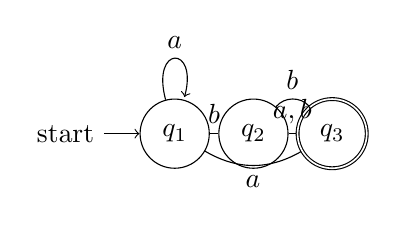
\begin{tikzpicture}
          \node[state, initial] (q1) {\(q_1\)};
          \node[state, right of=q1] (q2) {\(q_2\)};
          \node[state, accepting, right of=q2] (q3) {\(q_3\)};

          \draw
          (q1) edge[loop above] node{\(a\)} (q1)
          (q1) edge[above] node{\(b\)} (q2)
          (q2) edge[above] node{\(a,b\)} (q3)
          (q3) edge[bend right=50, above] node{\(b\)} (q2)
          (q3) edge[bend left, below] node{\(a\)} (q1);
        \end{tikzpicture}
      }

      \only<2> {
        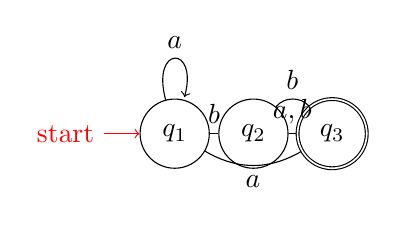
\begin{tikzpicture}[every initial by arrow/.style={red}]
          \node[state, initial] (q1) {\(q_1\)};
          \node[state, right of=q1] (q2) {\(q_2\)};
          \node[state, accepting, right of=q2] (q3) {\(q_3\)};

          \draw
          (q1) edge[loop above] node{\(a\)} (q1)
          (q1) edge[above] node{\(b\)} (q2)
          (q2) edge[above] node{\(a,b\)} (q3)
          (q3) edge[bend right=50, above] node{\(b\)} (q2)
          (q3) edge[bend left, below] node{\(a\)} (q1);
        \end{tikzpicture}
      }

      \only<3> {
        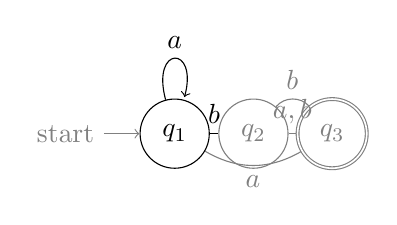
\begin{tikzpicture}[every initial by arrow/.style={gray}]
          \node[state, initial] (q1) {\(q_1\)};
          \node[state, right of=q1, gray] (q2) {\(q_2\)};
          \node[state, accepting, right of=q2, gray] (q3) {\(q_3\)};

          \draw
          (q1) edge[loop above] node{\(a\)} (q1)
          (q1) edge[above] node{\(b\)} (q2)
          (q2) edge[above, gray] node{\(a,b\)} (q3)
          (q3) edge[bend right=50, above, gray] node{\(b\)} (q2)
          (q3) edge[bend left, below, gray] node{\(a\)} (q1);
        \end{tikzpicture}
      }

      \only<4> {
        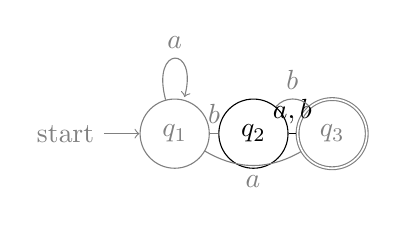
\begin{tikzpicture}[every initial by arrow/.style={gray}]
          \node[state, initial, gray] (q1) {\(q_1\)};
          \node[state, right of=q1] (q2) {\(q_2\)};
          \node[state, accepting, right of=q2, gray] (q3) {\(q_3\)};

          \draw
          (q1) edge[loop above, gray] node{\(a\)} (q1)
          (q1) edge[above, gray] node{\(b\)} (q2)
          (q2) edge[above] node{\(a,b\)} (q3)
          (q3) edge[bend right=50, above, gray] node{\(b\)} (q2)
          (q3) edge[bend left, below, gray] node{\(a\)} (q1);
        \end{tikzpicture}
      }

      \only<5> {
        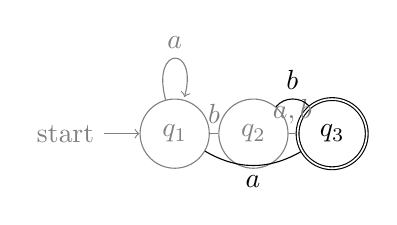
\begin{tikzpicture}[every initial by arrow/.style={gray}]
          \node[state, initial, gray] (q1) {\(q_1\)};
          \node[state, right of=q1, gray] (q2) {\(q_2\)};
          \node[state, accepting, right of=q2] (q3) {\(q_3\)};

          \draw
          (q1) edge[loop above, gray] node{\(a\)} (q1)
          (q1) edge[above, gray] node{\(b\)} (q2)
          (q2) edge[above, gray] node{\(a,b\)} (q3)
          (q3) edge[bend right=50, above] node{\(b\)} (q2)
          (q3) edge[bend left, below] node{\(a\)} (q1);
        \end{tikzpicture}
      }
    \end{center}
  \end{definition}
\end{frame}

\begin{frame}{\myframetitle}
  \begin{definition}[Automate minimal]
    L'automate \(M_1\) est << minimal >> du langage \(L = \{ab\}\)~:

    \begin{minipage}{0.47\textwidth}
      \centering
      \begin{tikzpicture}[node distance=2.5cm]
        \node[state, initial] (0) {\(0\)};
        \node[state, right of=0] (1) {\(1\)};
        \node[state, accepting, below of=1] (2) {\(2\)};

        \node[above =.75cm of $(0)!0.5!(1)$, align=center] {\(M_1\)};

        \draw
        (0) edge[above] node{\(a\)} (1)
        (1) edge[right] node{\(b\)} (2);
      \end{tikzpicture}
    \end{minipage}
    \hfill
    \begin{minipage}{0.47\textwidth}
      \centering
      \begin{tikzpicture}[node distance=2.5cm]
        \node[state, initial] (0) {\(0\)};
        \node[state, right of=0] (1) {\(1\)};
        \node[state, accepting, below of=1] (2) {\(2\)};
        \node[state, left of=2] (3) {\(3\)};

        \node[above =.75cm of $(0)!0.5!(1)$, align=center] {\(M_2\)};

        \draw
        (0) edge[above] node{\(a\)} (1)
        (1) edge[right] node{\(b\)} (2)
        (0) edge[left] node{\(a\)} (3);
      \end{tikzpicture}
    \end{minipage}
  \end{definition}
\end{frame}

\subsubsection{Lien entre les langages et les automates}

\setframetitle{Lien entre les langages et les automates}

\begin{frame}{\myframetitle}
  \begin{definition}[L'ensemble des langages reconnaisable]
    On définira l'ensemble des langages de \(\Sigma^*\) << reconnaissable >> par
    au moins un automate par \(\REC(\Sigma^*)\).
  \end{definition}

  \pause[]

  \begin{block}{Théorème de \textit{Kleene}}
    L'informaticien \textit{Stephen C. Kleene} a montré en 1956 que~:
    % LTeX: enabled=false
    \begin{align*}
      \REC(\Sigma^*) = \RAT(\Sigma^*)
    \end{align*}
    % LTeX: enabled=true
  \end{block}
\end{frame}

\subsubsection{Complexité en état}

\setframetitle{Complexité en état}

\begin{frame}{\myframetitle}
  \begin{definition}
    La << complexité en état >> est une mesure d'un \textbf{langage}, elle est
    définie comme le nombre d'états de l'automate minimal du langage~:

    \vphantom{}

    \begin{itemize}
      \item Complexité en état déterministe (qu'on notera \(C_{\det}\)).
      \item Complexité en état non déterministe (qu'on notera \(C_{\ndet}\)).
    \end{itemize}
  \end{definition}
\end{frame}

\begin{frame}{\myframetitle}
  \begin{example}[%
      \only<1>{Définition d'une famille}%
      \only<2>{\(C_{\ndet}(A_2) = 2 + 2\)}%
      \only<3>{\(C_{\det}(A_2) = 2^{2 + 1}\)}%
    ]
    \centering
    \vspace{-1.5\topsep}
    \begin{gather*}
      A_n = \Sigma^* \cdot a \cdot \Sigma^n
    \end{gather*}
    \vspace{-2.25\topsep}

    \onslide<2-> {
      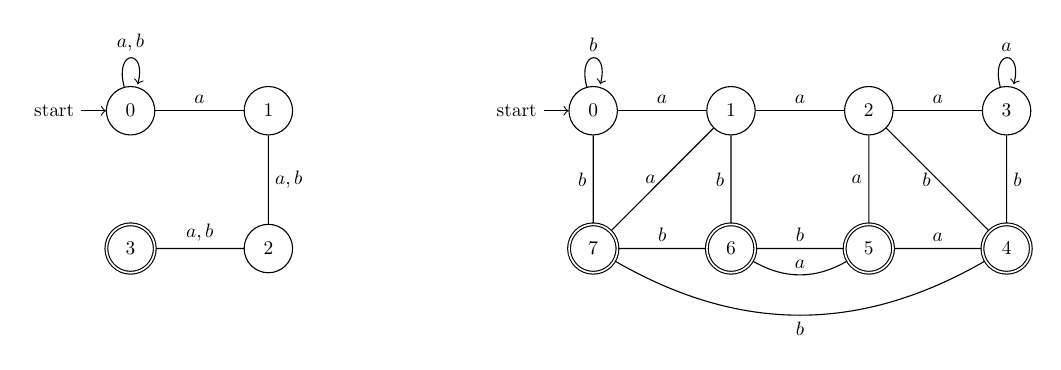
\begin{tikzpicture}[node distance=2.5cm, scale=0.7,transform shape]
        \node[state, initial] (0') {\(0\)};
        \node[state, right of=0'] (1') {\(1\)};
        \node[state, below of=1'] (2') {\(2\)};
        \node[state, accepting, left of=2'] (3') {\(3\)};

        \draw
        (0') edge[above] node{\(a\)} (1')
        (1') edge[right] node{\(a,b\)} (2')
        (2') edge[above] node{\(a,b\)} (3')
        (0') edge[loop above] node{\(a,b\)} (0');

        \onslide<3> {
          \node[state, initial, right =5cm of 1'] (0) {\(0\)};
          \node[state, right of=0] (1) {\(1\)};
          \node[state, right of=1] (2) {\(2\)};
          \node[state, right of=2] (3) {\(3\)};
          \node[state, accepting, below of=3] (4) {\(4\)};
          \node[state, accepting, left of=4] (5) {\(5\)};
          \node[state, accepting, left of=5] (6) {\(6\)};
          \node[state, accepting, left of=6] (7) {\(7\)};

          \draw
          (0) edge[loop above] node{\(b\)} (0)
          (3) edge[loop above] node{\(a\)} (3)

          (0) edge[above] node{\(a\)} (1)
          (1) edge[above] node{\(a\)} (2)
          (2) edge[above] node{\(a\)} (3)
          (3) edge[right] node{\(b\)} (4)
          (4) edge[above] node{\(a\)} (5)
          (5) edge[above] node{\(b\)} (6)
          (6) edge[above] node{\(b\)} (7)

          (1) edge[left] node{\(b\)} (6)
          (2) edge[left] node{\(b\)} (4)
          (4) edge[below, bend left] node{\(b\)} (7)
          (5) edge[left] node{\(a\)} (2)
          (6) edge[above, bend right] node{\(a\)} (5)
          (7) edge[left] node{\(a\)} (1)
          (7) edge[left] node{\(b\)} (0);
        }
      \end{tikzpicture}
    }
  \end{example}
\end{frame}

\begin{frame}{\myframetitle}
  \begin{definition}[Complexité en état opérationnielle]
    La fonction \(f\) à une complexité \(g(n, m)\) si~:
    \begin{center}
      \begin{tikzpicture}[transform shape, scale=0.8]
        \node[draw, ellipse, minimum width=1.5cm] (A) at (-2,2) {\(A\)};
        \node[draw, ellipse, minimum width=1.5cm] (B) at (2,2) {\(B\)};
        \node[draw, rectangle, minimum width=2cm, minimum height=1cm]
        (F) at (0,0) {\(f\)};
        \node[draw, ellipse, minimum width=1.5cm] (C) at (0,-2) {\(C\)};

        \node[left =0.25cm of A] {\(n\)};
        \node[right =0.25cm of B] {\(m\)};
        \node[below =0.25cm of C] {\(k \leq g(n, m)\)};

        \coordinate (center) at ($(F.north west)!0.5!(F.north east)$);

        \draw (A) -- (-0.5,2) -- ([shift={(-0.5cm,0cm)}] center);
        \draw (B) -- (0.5,2) -- ([shift={(0.5cm,0cm)}] center);
        \draw (F) -- (C);
      \end{tikzpicture}
    \end{center}
  \end{definition}
\end{frame}
\section{Préliminaires}

Dans cette section préliminaire, nous allons rappeler les notions
fondamentales nécessaires à la compréhension du reste du document. Nous y
définirons notamment les concepts d’alphabet, de mot, de langage, d’automate
et de complexité en nombre d’états. Ces définitions seront accompagnées
d’exemples et de remarques pour en faciliter l’assimilation

% ----------------------------------------------------------------------------
\subsection{Les mots}

\begin{definition}[Alphabet]
  Un \textit{alphabet} \(\Sigma\) est un ensemble fini non-vide de
  \textit{symboles}.
\end{definition}

\begin{definition}[Mot]
  Un \textit{mot} est une suite finie de symboles sur un alphabet \(\Sigma\).
  Le mot composé de zéro symbole est appelé mot vide et est noté 
  \(\varepsilon\). De plus, l'ensemble des mots sera noté \(\Sigma^*\)
\end{definition}

\begin{example}
  \vspace{-\baselineskip}
  \begin{align*}
    \Sigma &= \{a, b, c, d\}, \\
    w &= abbcdda.
  \end{align*}
\end{example}

\begin{definition}[Longueur d'un mot]
  On parlera de la \textit{longueur d'un mot} \(w\) noté \(\lvert w \rvert\)
  pour désigner le nombre de symboles qui le composent. 
\end{definition}

\begin{example}
  \vspace{-\baselineskip}
  \begin{align*}
    w &= abbcdda, \\
    \lvert w \rvert &= 7.
  \end{align*}
\end{example}

\begin{definition}[Concaténation de deux mots]
  On notera la \textit{concaténation} de deux mots \(u = a_0 \cdots a_n\) et 
  \(v = b_0 \cdots b_m\) par \(u \cdot v\). Qui est ainsi égal à \(u \cdot v =
  a_0 \cdots a_n b_0 \cdots b_m\). On notera que~:

  \vphantom{}

  \begin{itemize}
    \item[\bullet] La concaténation est associative \((w \cdot u) \cdot v = w
      \cdot (u \cdot v)\).
    \item[\bullet] La concaténation admet un élément neutre \(u \cdot 
      \varepsilon = \varepsilon \cdot u = u\).
  \end{itemize}
\end{definition}

\begin{example}
  \vspace{-\baselineskip}
  \begin{align*}
    u &= aba, \\
    v &= cdcd, \\
    u \cdot v &= abacdcd.
  \end{align*}
\end{example}

\begin{definition}[Facteur, préfixe, suffixe d'un mot]
  Un \textit{facteur} \(u\) d'un mot \(w\) est une suite extraite de la suite
  de lettre qui composent le mot \(w\)~:
  \begin{align*}
    u \text{ est un facteur de } w \Longleftrightarrow \exists (v, x) \in
    (\Sigma ^ *)^2 ~|~ w = v \cdot u \cdot x.
  \end{align*} 

  \begin{itemize}
    \item[\bullet] Par ailleurs, on parlera de \textit{préfixe} quand \(v = 
      \varepsilon\).
    \item[\bullet] Enfin, on parlera de \textit{suffixe} quand \(x =
      \varepsilon\).
  \end{itemize}

  \vphantom{}

  Par ailleurs, on remarquera que \(\varepsilon\) est~: \textit{préfixe}, 
  \textit{suffixe} et \textit{facteur} de tout mot.
\end{definition}

\begin{example}
  Dans cet exemple, on a que \(u\) est un facteur de \(w\), que \(v\) est un
  préfixe de \(w\) et enfin que \(y\) est un suffixe de \(w\)~:
  \begin{align*}
    w &= abbcdda, \\
    u &= bcd, \\
    v &= abb, \\
    y &= dda.
  \end{align*}
\end{example}

\begin{definition}[Le miroir d'un mot]
  Le \textit{miroir} d'un mot \(w\) noté \(\overleftarrow{w}\). Qui est ainsi
  défini récursivement comme ceci~:
  \begin{align*}
    \overleftarrow{\varepsilon} &= \varepsilon, \\
    \overleftarrow{u \cdot a} &= a \cdot \overleftarrow{u}, \\
    \text{Avec } a \in~&\Sigma \text{ et } u \in \Sigma^*.
  \end{align*}
\end{definition}

\begin{example}
  \vspace{-\baselineskip}
  \begin{align*}
    w &= abbcdda, \\
    \overleftarrow{w} &= addcbba.
  \end{align*}
\end{example}

% ----------------------------------------------------------------------------
\subsection{Les langages}

\begin{definition}[Langage]
  Un \textit{langage} \(L\) est un ensemble de mots sur un alphabet fini
  \(\Sigma\). On appellera \textit{langage vide} le langage ne comportant
  aucun mot et sera noté \(\varnothing\).
\end{definition}

\begin{example}
  \vspace{-\baselineskip}
  \begin{align*}
    \Sigma &= \{a, b, c, d\}, \\
    L_1 &= \{a, aa, bc, da, \varepsilon\}, \\
    L_2 &= \varnothing.
  \end{align*}
\end{example}

\begin{definition}[L'union de langages]
  L'\textit{union} de deux langages sera notée \(L_1 \cup L_2\) et est définie
  comme ceci~:
  \begin{gather*}
      L_1 \cup L_2 = \{w \in \Sigma ^ * \mid w \in L_1 \lor w \in L_2\}.
  \end{gather*}
\end{definition}

\begin{example}
  \vspace{-\baselineskip}
  \begin{align*}
    L_1 &= \{\varepsilon, a, aa, bc, da\}, \\
    L_2 &= \{d, aa, cd\}, \\
    L_1 \cup L_2 &= \{\varepsilon, a, d, aa, cd, bc, da\}. \\
  \end{align*}
\end{example}

\begin{definition}[Concaténation de langages]
  La \textit{concaténation} de deux langages sera notée \(L_1 \cdot L_2\) et
  est définie grâce à la concaténation des mots qui composent les langages~:
  \begin{gather*}
    L_1 \cdot L_2 = \{u \cdot v ~|~ u \in L_1, v \in L_2\}.
  \end{gather*}
\end{definition}

\begin{example}
  \vspace{-\baselineskip}
  \begin{align*}
    L_1 &= \{\varepsilon, a, aa\}, \\
    L_2 &= \{d, cc\}, \\
    L_1 \cdot L_2 &= \{d, ad, aad, cc, acc, aacc\}.
  \end{align*}
\end{example}

\begin{definition}[Copie n-ième d'un langage]
  La \textit{copie n-ième} d'un langage \(L\) notée \(L^n\) et est définie
  récursivement comme ceci~:
  \begin{align*}
    L^0 &= \{\varepsilon\}, \\
    L^n &= L^{n - 1} \cdot L.
  \end{align*}
\end{definition}

\begin{example}
  \vspace{-\baselineskip}
  \begin{align*}
    L &= \{\varepsilon, a\}, \\
    L^3 &= \{\varepsilon, a, aa, aaa\}.
  \end{align*}
\end{example}

\begin{definition}[L'étoile (de \textsc{Kleene}) d'un langage]
  L'\textit{étoile} (de \textsc{Kleene}) d'un langage noté \(L^*\), sera
  définie comme ceci~:
  \begin{gather*}
    L^* = \bigcup_{i \geq 0} L^i.
  \end{gather*}
\end{definition}

\begin{example}
  \vspace{-\baselineskip}
  \begin{align*}
    L &= \{a\}, \\
    L^* &= \{\varepsilon\} \cup \{a\} \cup \{aa\} \cup \cdots
  \end{align*}
\end{example}

\begin{remark}
  Grâce à cette opération, on comprend dorénavant la notion \(\Sigma^*\) comme
  l'ensemble des mots de l'alphabet \(\Sigma\), il pourra donc aussi être vu
  comme le langage contenant tous les mots.
\end{remark}

\begin{definition}[Langages rationnel]
  On note \(Rat(\Sigma^*)\) le plus petit ensemble de langages sur
  \(\Sigma^*\) vérifiant les propriétés suivantes~:

  \vphantom{}

  \begin{itemize}
    \item[\bullet] \(\varnothing \in Rat(\Sigma^*)\).
    \item[\bullet] \(\{a\} \in Rat(\Sigma^*) \text{ avec } a \in \Sigma\).
    \item[\bullet] \(Rat(\Sigma^*)\) est fermé pour les opérations d'union,
    de concaténation et pour l'étoile.
  \end{itemize}
\end{definition}

\begin{remark}
  Pour simplifier l’écriture, nous écrirons \(+\) pour représenter l’union, et
  nous utiliserons également \(ab\) au lieu de \(\{ab\}\).
\end{remark}

\begin{example}
  \vspace{-\baselineskip}
  \begin{align*}
    L = \varnothing + (a^* \cdot (b + \varepsilon)).
  \end{align*}
\end{example}

% ----------------------------------------------------------------------------
\subsection{Les automates}

Nous allons parler des automates sans \(\varepsilon\)-transition (des 
automates utilisent des \\\(\varepsilon\)-transitions, comme ceux de 
\textsc{Thompson} \cite{thompson1968programming}, utilisés par nos 
ordinateurs). Pour autant, les automates que nous verrons ne sont pas limités
par le manque de ces transitions.

\begin{definition}[Automate]
  Un \textit{automate} est un objet mathématique \textit{reconnaissant} un
  langage. On notera \(M \in AFN(\Sigma, \eta)\) l'automate qui a pour
  \textit{transition} des valeurs dans \(\Sigma\), des valeurs d'\textit{état}
  dans \(\eta\).

  \vphantom{}

  On aura aussi, \(AFN(\Sigma, \eta)\), l'ensemble des automates finis 
  \textit{non déterministes} de valeur de transition dans \(\Sigma\) et de 
  valeur d'état dans \(\eta\). Enfin, on écrira \(L(M)\) pour désigner le
  langage qu'il reconnait.

  \vphantom{}

  Un automate est un tuple qu'on peut écrire de cette forme \(M = (Q, I, F, 
  \delta)\) avec~:
  \begin{alignat*}{3}
    &\cmath{Q} && \subseteq \eta &&\text{États de l'automate.} \\
    &\cmath{I} && \subseteq Q &&\text{États initiaux.} \\
    &\cmath{F} && \subseteq Q &&\text{États finaux.} \\
    &\cmath{\delta}&&: Q \times \Sigma \to \mathcal{P}(Q)~ &&\text{Fonction de
    transition.}
  \end{alignat*}
\end{definition}

\begin{remark}[Extension de la fonction de transition]
  On peut étendre la fonction de transition pour ce qu’elle prenne en entrée
  non plus un simple symbole, mais un mot. Sa signature devient alors 
  \(\delta~: Q \times \Sigma^* \to \mathcal{P}(Q)\), et elle est définie comme
  suit~:
  \begin{align*}
    \delta(q, \varepsilon) &= \{q\}, \\
    \delta(q, a \cdot w) &= \bigcup_{p \in \delta(q, a)} \delta(p, w),
    \text{ avec } a \in \Sigma.
  \end{align*}
\end{remark}

\begin{definition}[Reconnaissance d'un mot par un automate]
  Un mot est \textit{reconnu} (ou \textit{accepté}) s'il existe une suite de
  transition partant d'un état initial vers un état final~:
  \begin{align*}
    w \text{ est accepté par } M \Longleftrightarrow \left( \bigcup_{i \in I}
    \delta(i, w) \right) \cap F \neq \varnothing.
  \end{align*}
\end{definition}

\begin{definition}[Langage d'un automate]
  Le \textit{langage d'un automate} est donc l'ensemble des mots qu'il
  reconnait~:
  \begin{align*}
    L(M) = \{w \in \Sigma^* \mid w \text{ est accepté par } M\}.
  \end{align*}
\end{definition}

\begin{example}[Représentation d'un automate]
  Un automate peut se représenter à l'aide d'un graphe orienté et valué
  particulier. Par exemple, si on veut représenter \(M = (\{q_1, q_2, q_3,
  q_4, q_5\}, \{q_1, q_2\},\{q_2, q_3\}, \delta)\) avec \(M \in AFN(\Sigma,
  \eta)\), \(\Sigma = \{a, b\}\), \(\eta = \{q_1, q_2, q_3, q_4, q_5\}\) et
  \(\delta\) défini comme ceci~:
  \begin{align*}
    \delta(q_1, a) &= \{q_2, q_4\}, & \delta(q_3, b) & = \{q_4\}, \\
    \delta(q_1, b) &= \varnothing,  & \delta(q_4, a) & = \{q_5\}, \\
    \delta(q_2, a) &= \varnothing,  & \delta(q_4, b) & = \{q_3\}, \\
    \delta(q_2, b) &= \varnothing,  & \delta(q_5, a) & = \{q_4\}, \\
    \delta(q_3, a) &= \{q_3\},      & \delta(q_5, b) & = \{q_5\}.
  \end{align*}
  \begin{figure}[H]
    \centering
    \captionsetup{type=figure,justification=centering}
    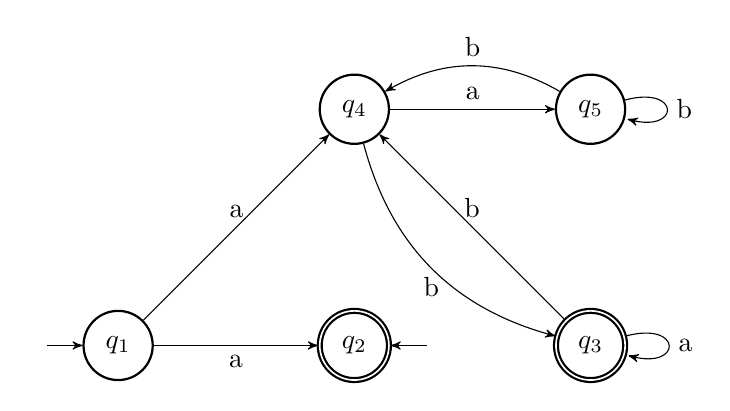
\begin{tikzpicture}
      \tikzset{
        ->,
        >=stealth',
        node distance=3cm,
        every state/.style={thick},
        initial text=$ $,
      }
      \node[state, initial] (q1) {\(q_1\)};
      \node[state, initial right, accepting, right of=q1] (q2) {\(q_2\)};
      \node[state, above of=q2] (q4) {\(q_4\)};
      \node[state, accepting, right of=q2] (q3) {\(q_3\)};
      \node[state, right of=q4] (q5) {\(q_5\)};

      \draw
        (q1) edge[above] node{a} (q4)
        (q1) edge[below] node{a} (q2)
        (q4) edge[bend right, below] node{b} (q3)
        (q4) edge[above] node{a} (q5)
        (q3) edge[above] node{b} (q4)
        (q3) edge[loop right] node{a} (q3)
        (q5) edge[bend right, above] node{b} (q4)
        (q5) edge[loop right] node{b} (q5);
    \end{tikzpicture}
    \caption{Exemple de représentation graphique d'un automate.}
  \end{figure}

  On peut voir que les états initiaux ont une petite flèche qui pointe sur eux
  et que les états finaux ont un double contour. Et, que les transitions sont
  symbolisées par des flèches entre les états et que ces flèches sont 
  labellisées.
\end{example}

\begin{definition}[Automate déterministe]
  Un automate est dit \textit{déterministe} quand tous ses états vont au
  maximum à un état par symbole et que l'automate ne possède qu'un seul état
  initial.
  \begin{gather*}
    \lvert I \rvert = 1 \land \forall q \in Q, \forall a \in \Sigma, \lvert 
    \delta(q, a) \rvert \leq 1 \Longleftrightarrow M \in DFA(\Sigma, \eta)
  \end{gather*}
  avec \(DFA(\Sigma, \eta)\) l'ensemble des automates déterministe.
\end{definition}

\begin{example}[Représentation d'un automate déterministe]
  \vspace{-\baselineskip}
  \begin{figure}[H]
    \centering
    \captionsetup{type=figure,justification=centering}
    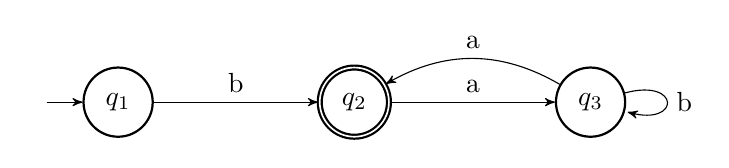
\begin{tikzpicture}
      \tikzset{
        ->,
        >=stealth',
        node distance=3cm,
        every state/.style={thick},
        initial text=$ $,
      }
      \node[state, initial] (q1) {\(q_1\)};
      \node[state, accepting, right of=q1] (q2) {\(q_2\)};
      \node[state, right of=q2] (q3) {\(q_3\)};

      \draw
        (q1) edge[above] node{b} (q2)
        (q2) edge[above] node{a} (q3)
        (q3) edge[bend right, above] node{a} (q2)
        (q3) edge[loop right] node{b} (q3);
    \end{tikzpicture}
    \caption{Exemple de représentation graphique d'un automate déterministe.}
  \end{figure}
\end{example}

\begin{definition}[L'ensemble des langages reconnaissable]
  On note \(Rec(\Sigma^*)\), l'ensemble des langages de \(\Sigma^*\) dit 
  \textit{reconnaissable}~:
  \begin{align*}
    L \in Rec(\Sigma^*) \Longleftrightarrow \exists M \in NFA(\Sigma, \eta)
    \land L = L(M).
  \end{align*}
\end{definition}

\begin{theorem}[Théorème de \textsc{Kleene}]
  Le mathématicien \textsc{Stephen Cole Kleene} a démontré que~:
  \begin{align*}
    Rec(\Sigma^*) = Rat(\Sigma^*).
  \end{align*}
  On pourra alors passer de langage rationnel à automate et vice-versa.
\end{theorem}

\begin{remark}
  La notation \(\lvert M \rvert\) représentera le nombre d'états de l'automate
  \(M\).
\end{remark}

\begin{definition}[Automate minimal]
  Un automate est dit \textit{minimal} lorsqu’il s’agit de l’automate ayant le
  plus petit nombre d’états possible qui reconnaît un langage donné~:
  \begin{align*}
    M \text{ est minimal} \Longrightarrow \nexists N \in NFA(\Sigma, \eta)
    \land L(M) = L(N).
  \end{align*}
  On parlera d'automate \text{déterministe minimal} quand~:
    \begin{align*}
    M \text{ est déterministe minimal} \Longrightarrow \nexists N \in 
    DFA(\Sigma, \eta) \land L(M) = L(N).
  \end{align*}
\end{definition}

\begin{example}[Représentation d'un automate minimal]
  Dans cet exemple, l'automate \(M_2\) est bien plus petit que l'automate
  \(M_1\), c'est même le plus petit automate reconnaissant leur langage
  (\(a^*\))
  \begin{figure}[H]
    \centering
    \captionsetup{type=figure,justification=centering}
    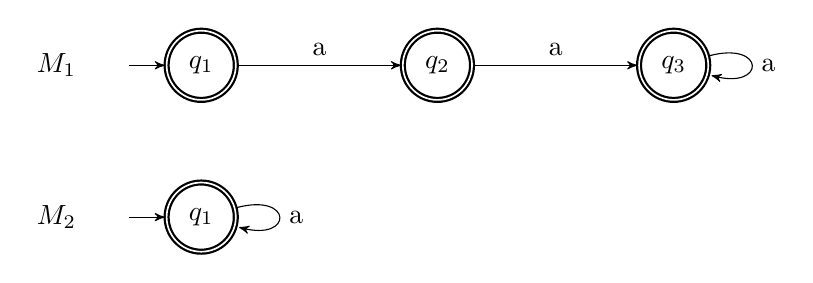
\begin{tikzpicture}
      \tikzset{
        ->,
        >=stealth',
        node distance=3cm,
        every state/.style={thick},
        initial text=$ $,
      }
      \node[state, initial, accepting] (q1) {\(q_1\)};
      \node[left=1cm of q1] {\(M_1\)};
      \node[state, accepting, right of=q1] (q2) {\(q_2\)};
      \node[state, accepting, right of=q2] (q3) {\(q_3\)};
      \node[state, initial, accepting, below=1cm of q1] (q4) {\(q_1\)};
      \node[left=1cm of q4] {\(M_2\)};

      \draw
        (q1) edge[above] node{a} (q2)
        (q2) edge[above] node{a} (q3)
        (q3) edge[loop right] node{a} (q3)
        (q4) edge[loop right] node{a} (q4);
    \end{tikzpicture}
    \caption{
      Exemple de représentation graphique d'un automate minimal.
    }\label{fig:ex_minimal}
  \end{figure}
\end{example}

%-----------------------------------------------------------------------------
\subsection{La complexité en état}

\begin{definition}[Complexité en état d'un langage (rationnel)]
  La \textit{complexité en état} d'un langage est le nombre d'états de
  l'automate minimal reconnaissant ce langage~:
  \begin{gather*}
    \mathcal{C}(L) = \lvert M \rvert \land L(M) = L \text{ avec} \\ 
    M \text{ est un automate minimal.}
  \end{gather*}
  Cette complexité se scinde en deux parties~:

  \vphantom{}

  \begin{itemize}
    \item[\bullet] La complexité non déterministe (\(\mathcal{C}_{ndet}\))
    quand~:
    \begin{align*}
      M \in NFA(\Sigma, \eta).
    \end{align*}
    \item[\bullet] La complexité déterministe (\(\mathcal{C}_{det}\))
    lorsque~:
    \begin{align*}
      M \in DFA(\Sigma, \eta).
    \end{align*}
  \end{itemize}
\end{definition}

\begin{example}
  Si on reprend le langage de la figure~\ref{fig:ex_minimal}, \(M_2\) est
  l'automate minimal reconnaissant \(a^*\) et il n'a qu'un état, de ce fait ce
  langage à une complexité en état déterministe de \(1\). Et, donc aussi, une
  complexité non déterministe de \(1\), puisque tout automate déterministe est
  dans \(NFA(\Sigma, \eta)\) et qu'on ne peut pas faire un automate à moins
  d'un état.
\end{example}

\begin{definition}[Complexité en état opérationnel]
  La \textit{complexité en état opérationnel} peut être vu comme la borne
  supérieure de la complexité en état du langage produit par l'opération.
  Autrement dit, \(f\) a une complexité de \(g(n_1, \ldots, n_k)\) quand~:
  \begin{align*}
    \forall (L_1, \ldots, L_k) \in \mathcal{P}(\Sigma^*) \quad
    \mathcal{C}(f(L_1, \ldots, L_k)) \leq 
    g(\mathcal{C}(L_1), \ldots, \mathcal{C}(L_k)).
  \end{align*}
  De même que la complexité en état, la complexité en état opérationnel se
  scinde en deux parties~:

  \vphantom{}

  \begin{itemize}
    \item[\bullet] La complexité non déterministe quand~:
    \begin{align*}
      \mathcal{C}_{ndet}(f(L_1, \ldots, L_k)) \leq 
      g(\mathcal{C}_{ndet}(L_1), \ldots, \mathcal{C}_{ndet}(L_k)).
    \end{align*}
    \item[\bullet] La complexité déterministe lorsque~:
    \begin{align*}
      \mathcal{C}_{det}(f(L_1, \ldots, L_k)) \leq 
      g(\mathcal{C}_{det}(L_1), \ldots, \mathcal{C}_{det}(L_k)).
    \end{align*}
  \end{itemize}
\end{definition}

\begin{remark}
  La complexité en état déterministe sera toujours supérieure ou égale à la
  complexité en état non déterministe, dû au fait que les automates
  déterministes sont aussi des automates non déterministe, mais avec des
  contraintes en plus.
\end{remark}

\begin{example}
  Voici quelques complexités en état opérationnel connues et importantes~:
  \begin{table}[H]
    \centering
    \captionsetup{type=table,justification=centering}
    \renewcommand{\arraystretch}{2}
    \begin{tabular}{|c|c|c|}
    \hline
      \textbf{Fonction} & \textbf{Complexité} & \textbf{Source} \\
      \hline
      L'union non déterministe & \(m + n\) & \textsc{Holzer} et 
      \textsc{Kutrib}~\cite{holzer_kutrib} \\
      \hline
      L'union déterministe & \(m n\) & 
      \textsc{Maslov}~\cite{maslov1970estimates} \\
      \hline
      L'intersection non déterministe & \(m n\) & \textsc{Holzer} et 
      \textsc{Kutrib}~\cite{holzer_kutrib} \\
      \hline
      L'intersection déterministe & \(m n\) & 
      \textsc{Maslov}~\cite{maslov1970estimates} \\
      \hline
      La concaténation non déterministe & \(m + n\) & \textsc{Holzer} et 
      \textsc{Kutrib}~\cite{holzer_kutrib} \\
      \hline
      La concaténation déterministe & \(m 2^n - 2^{n - 1}\) & 
      \textsc{Maslov}~\cite{maslov1970estimates} \\
      \hline
      L'étoile (de \textsc{Kleene}) non déterministe & \(n + 1\) &
      \textsc{Holzer} et \textsc{Kutrib}~\cite{holzer_kutrib} \\
      \hline
      L'étoile (de \textsc{Kleene}) déterministe & \(\frac{3}{4}2^n\) & 
      \textsc{Maslov}~\cite{maslov1970estimates} \\
      \hline
    \end{tabular}
    \caption{
      Tableau de complexité en état opérationnel de plusieurs opérations.
    }
  \end{table}
\end{example}

\begin{remark}[Complexité de la déterminisation]
  L'opération de \textit{déterminisation}, c'est-à-dire l'opération de rendre
  un automate non déterministe quelconque en un automate déterministe à une
  complexité en état de \(2^n\).

  Même si cette opération ne rentre pas réellement dans notre définition de la
  complexité en état, car prenant en entrée un automate non déterministe et
  renvoyant un automate déterministe.
\end{remark}

\section{Le trognon d'un langage}

\subsection{Définition}

\setframetitle{Définition}

\begin{frame}{\myframetitle}
  \begin{block}{Le trognon d'un mot}
    \centering
    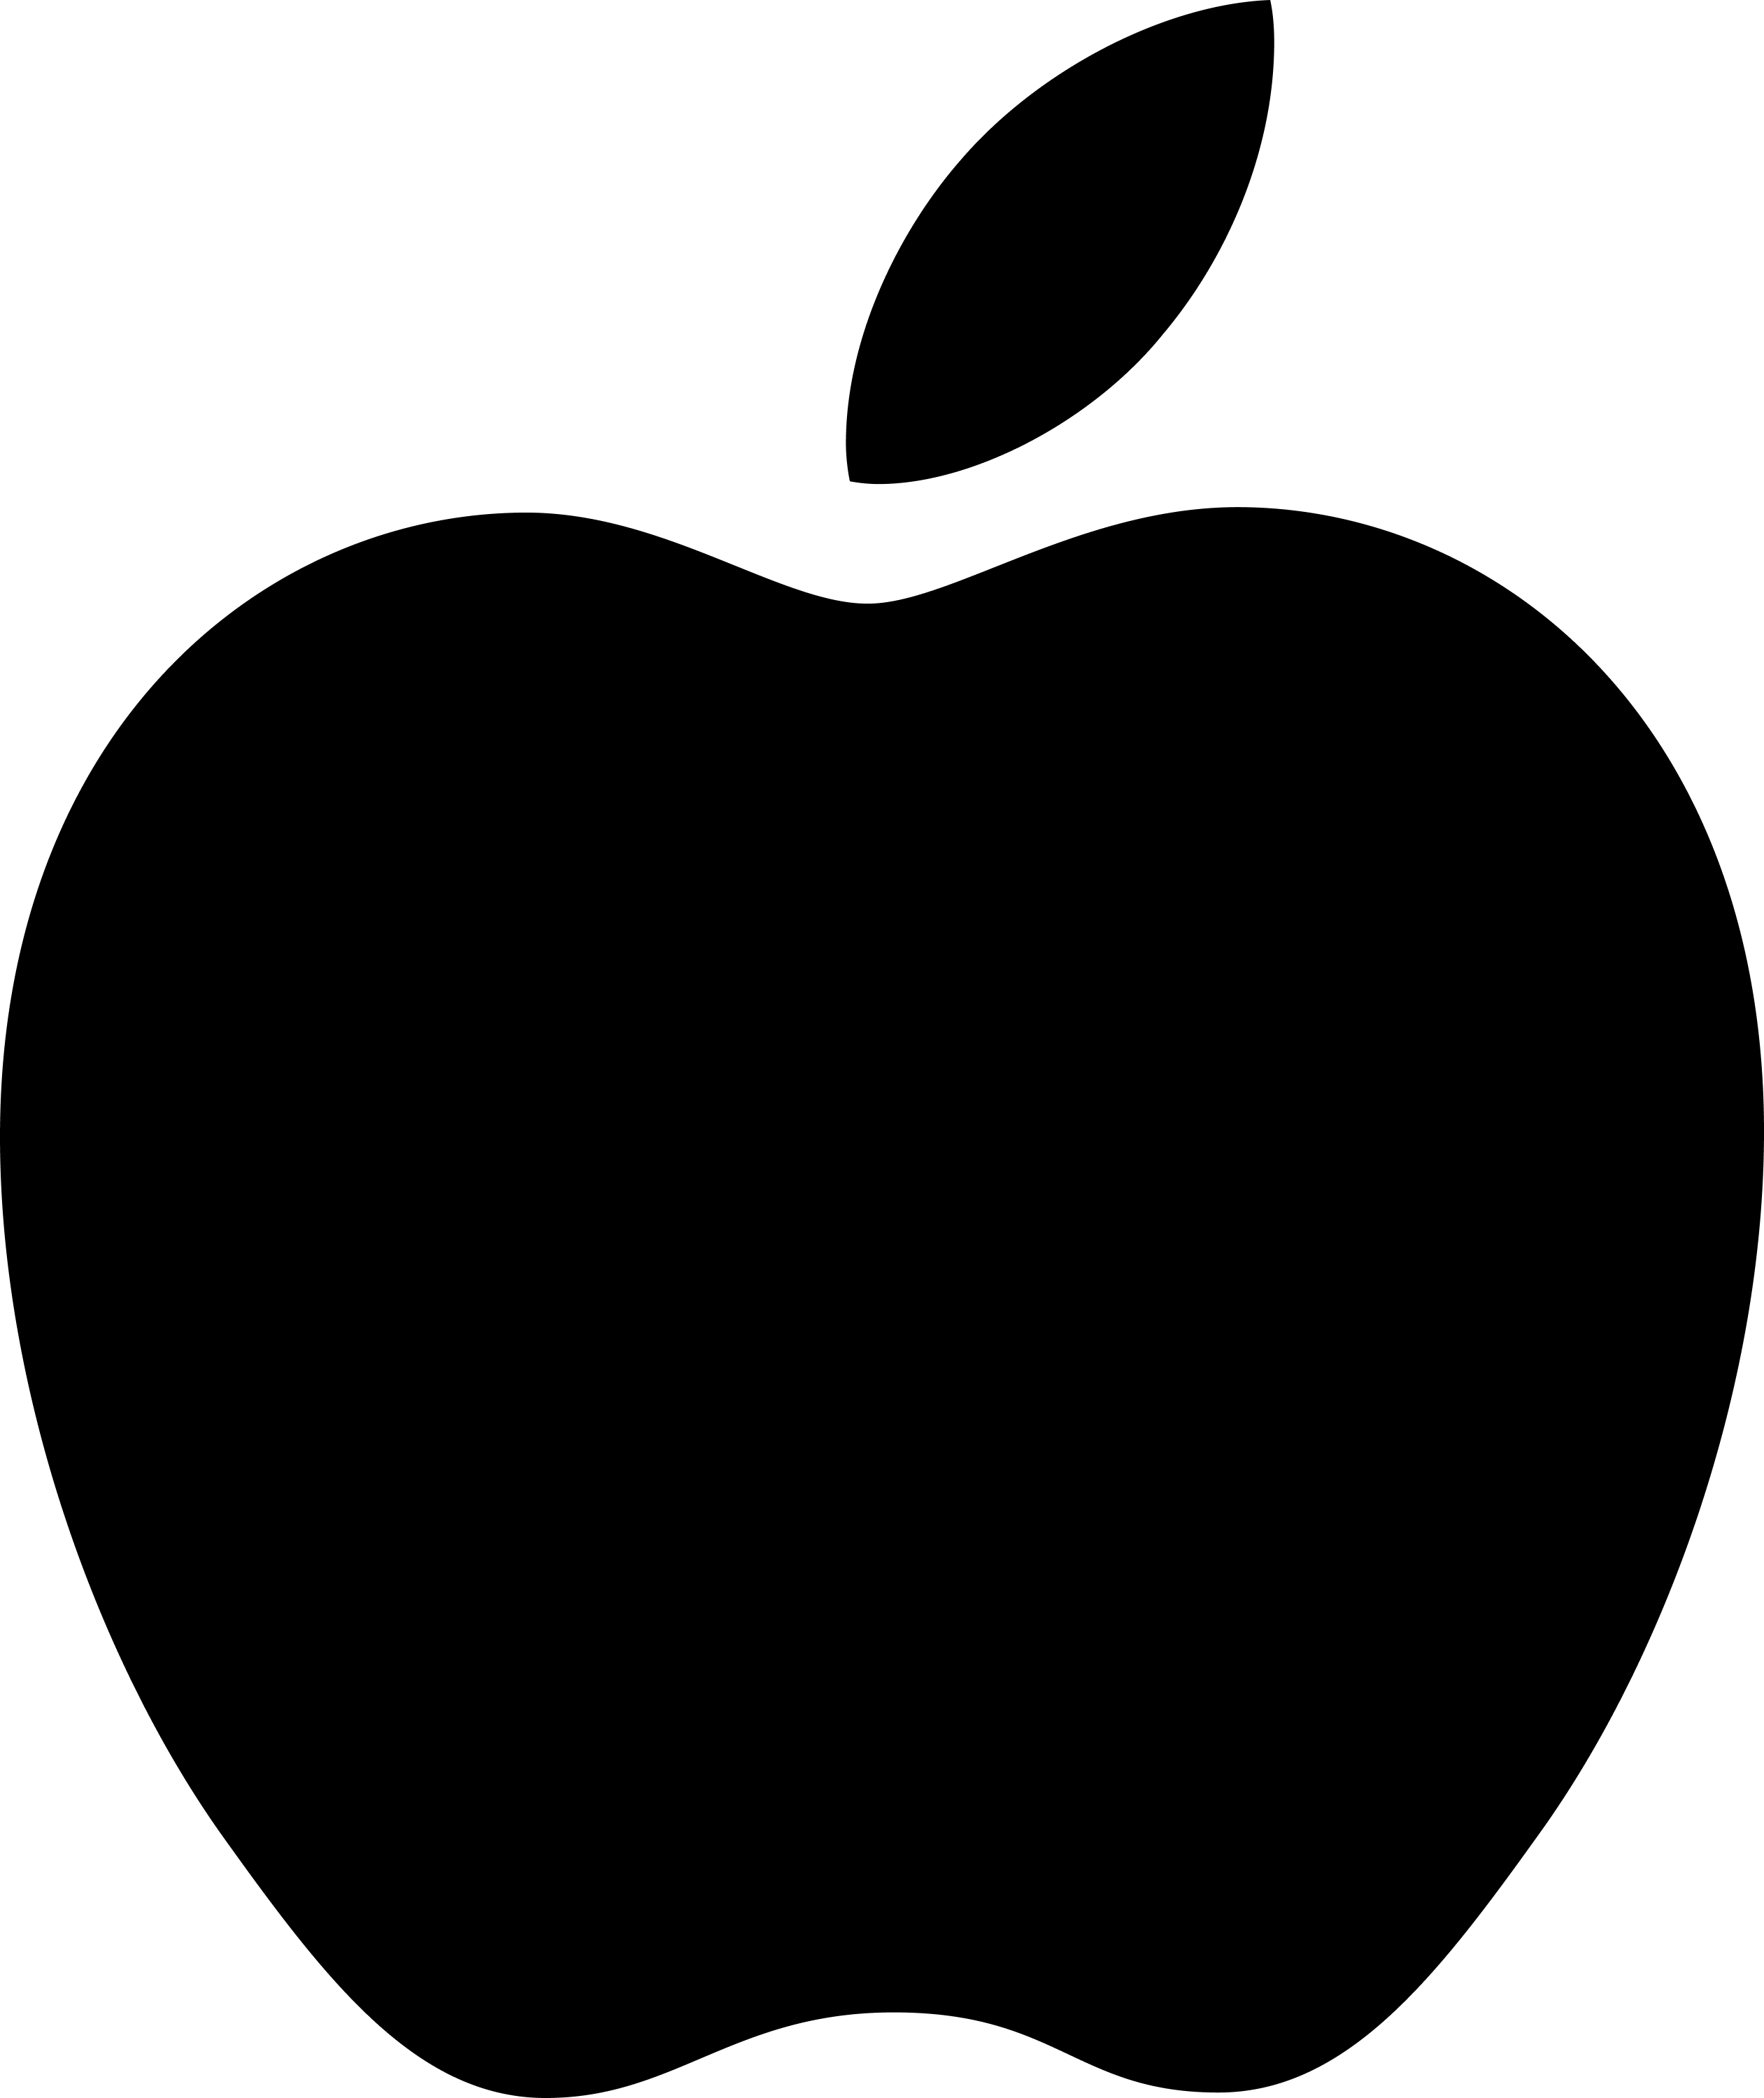
\includegraphics[width=0.25\textwidth]{./resources/full_apple.png}

    \pause[]

    \vphantom{}

    \Large{\(abcdcba\)}
  \end{block}
\end{frame}

\begin{frame}{\myframetitle}
  \begin{block}{Le trognon d'un mot}
    \centering
    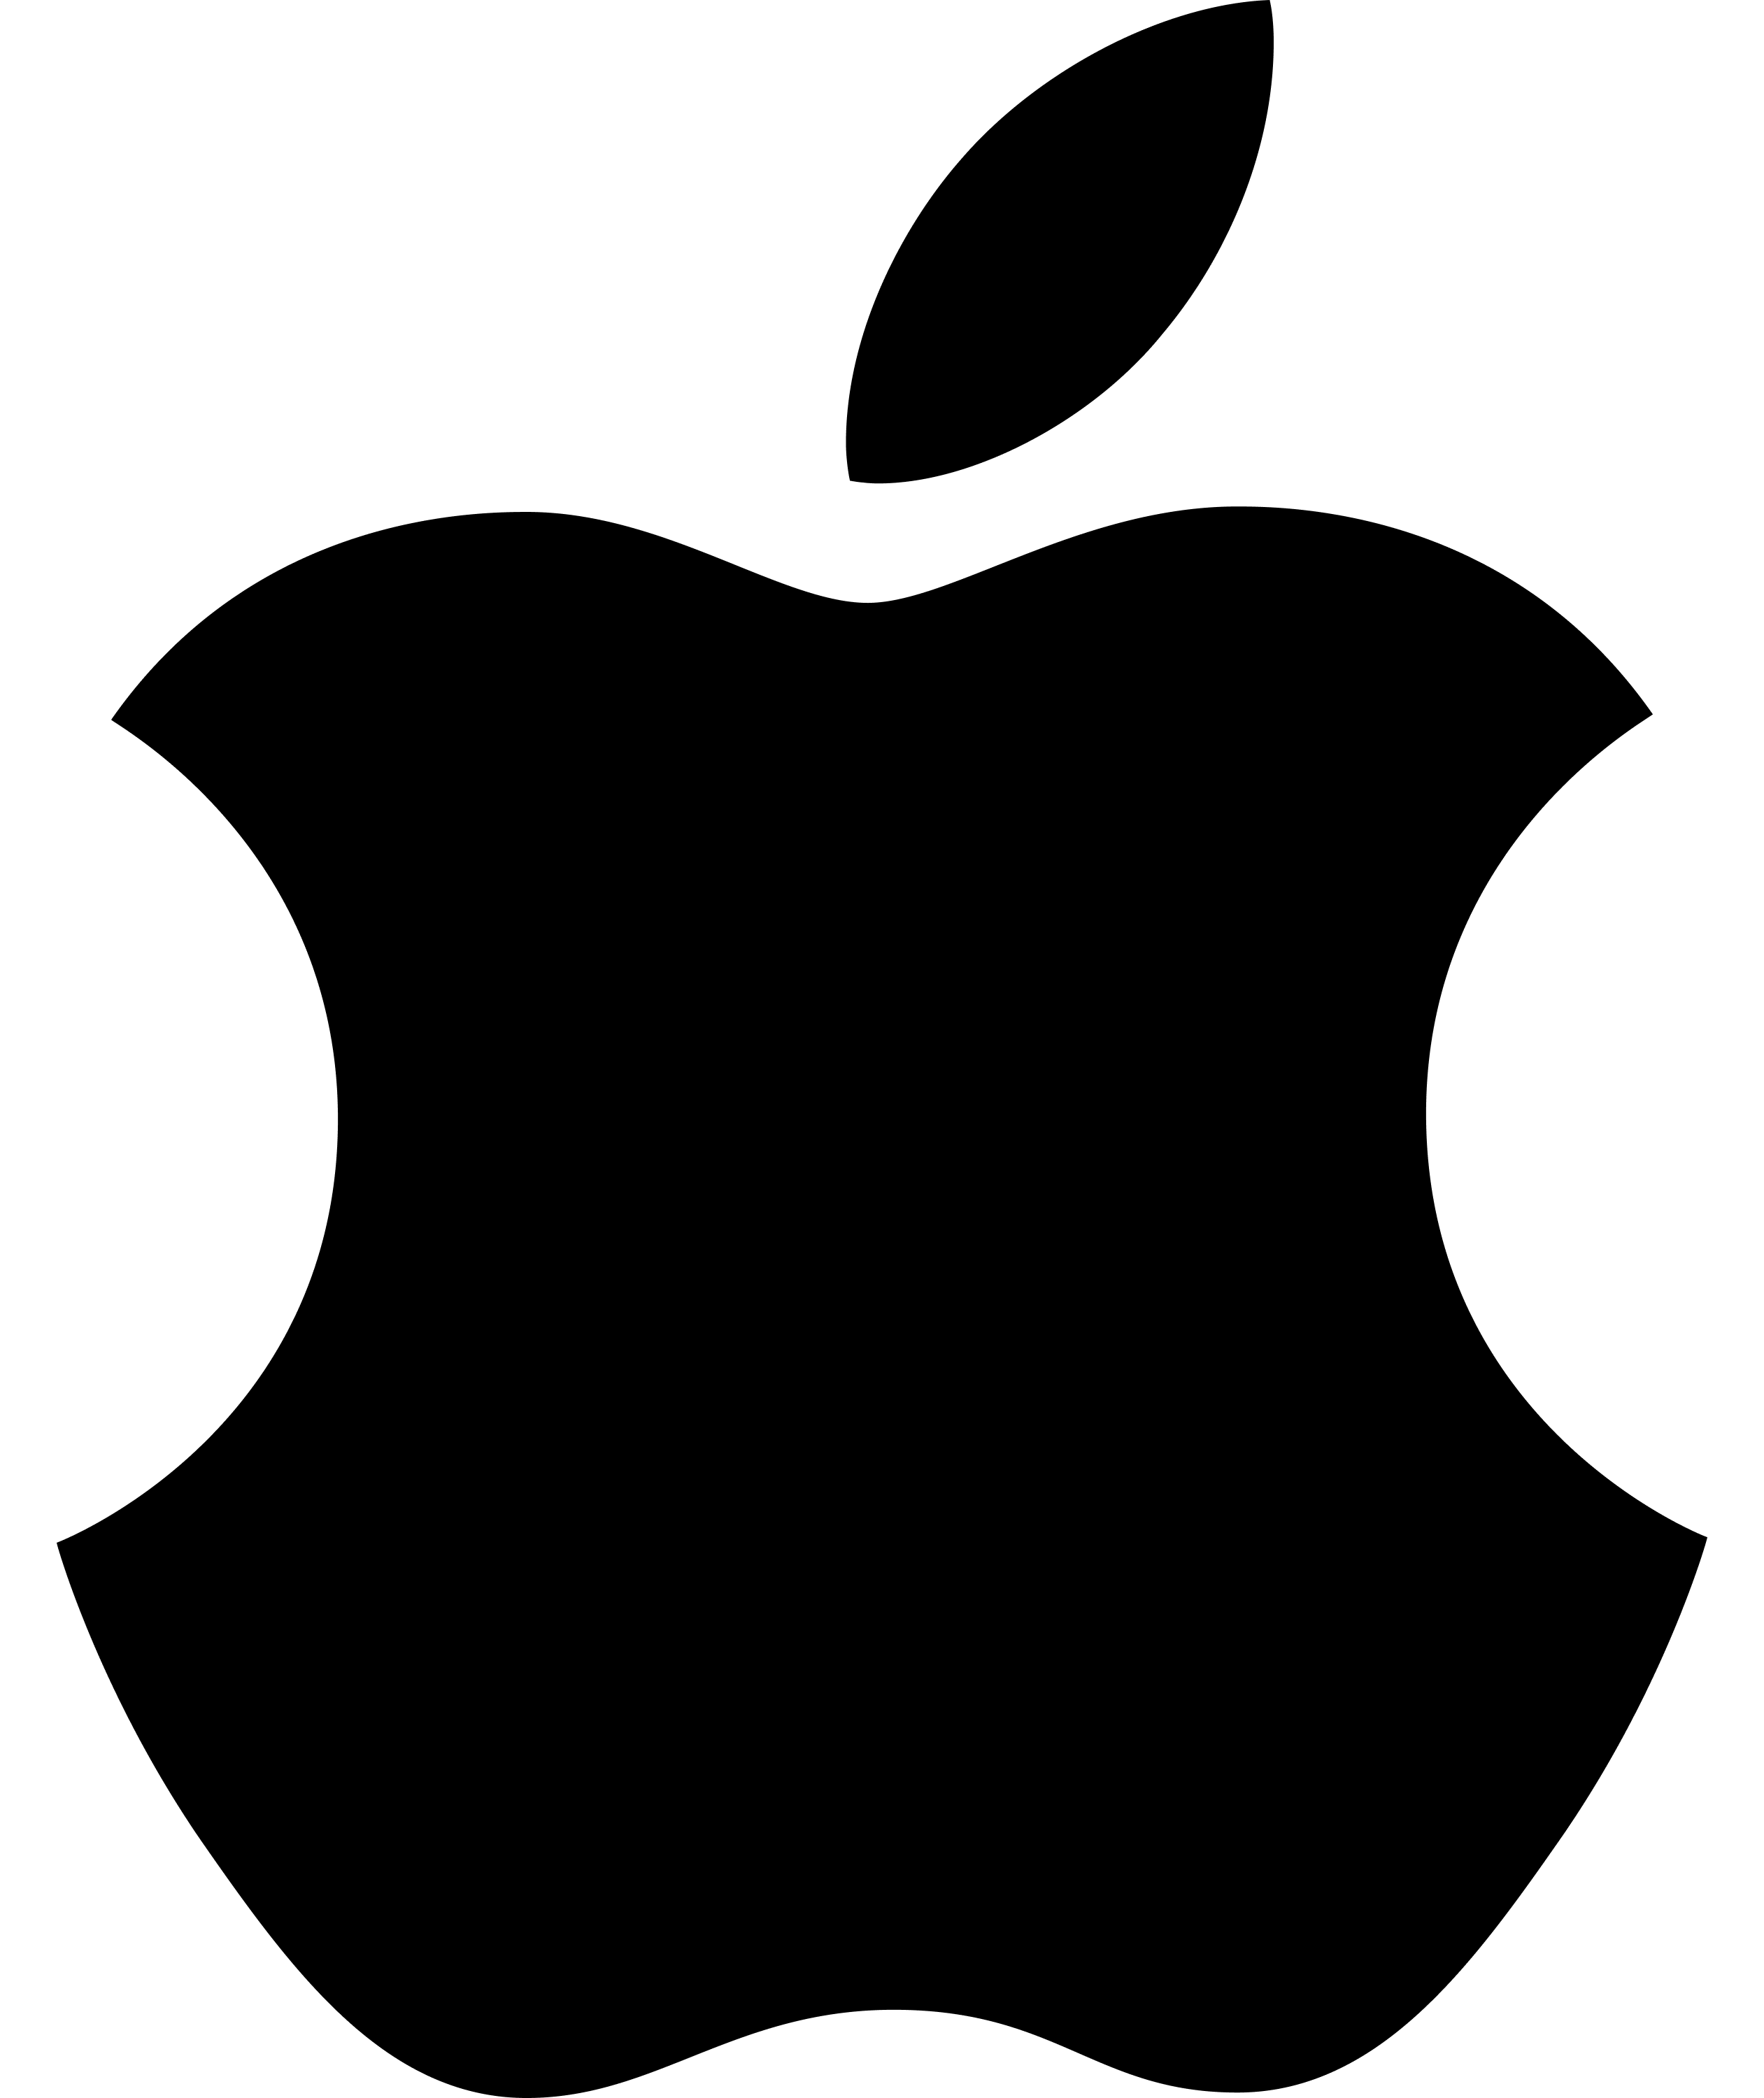
\includegraphics[width=0.25\textwidth]{./resources/mid_apple.png}

    \pause[]

    \vphantom{}

    \Large{\(\color{red}{ab} \color{black}{\cdot cdc \cdot} \color{red}{ba}\)}
  \end{block}
\end{frame}

\begin{frame}{\myframetitle}
  \begin{block}{Le trognon d'un mot}
    \centering
    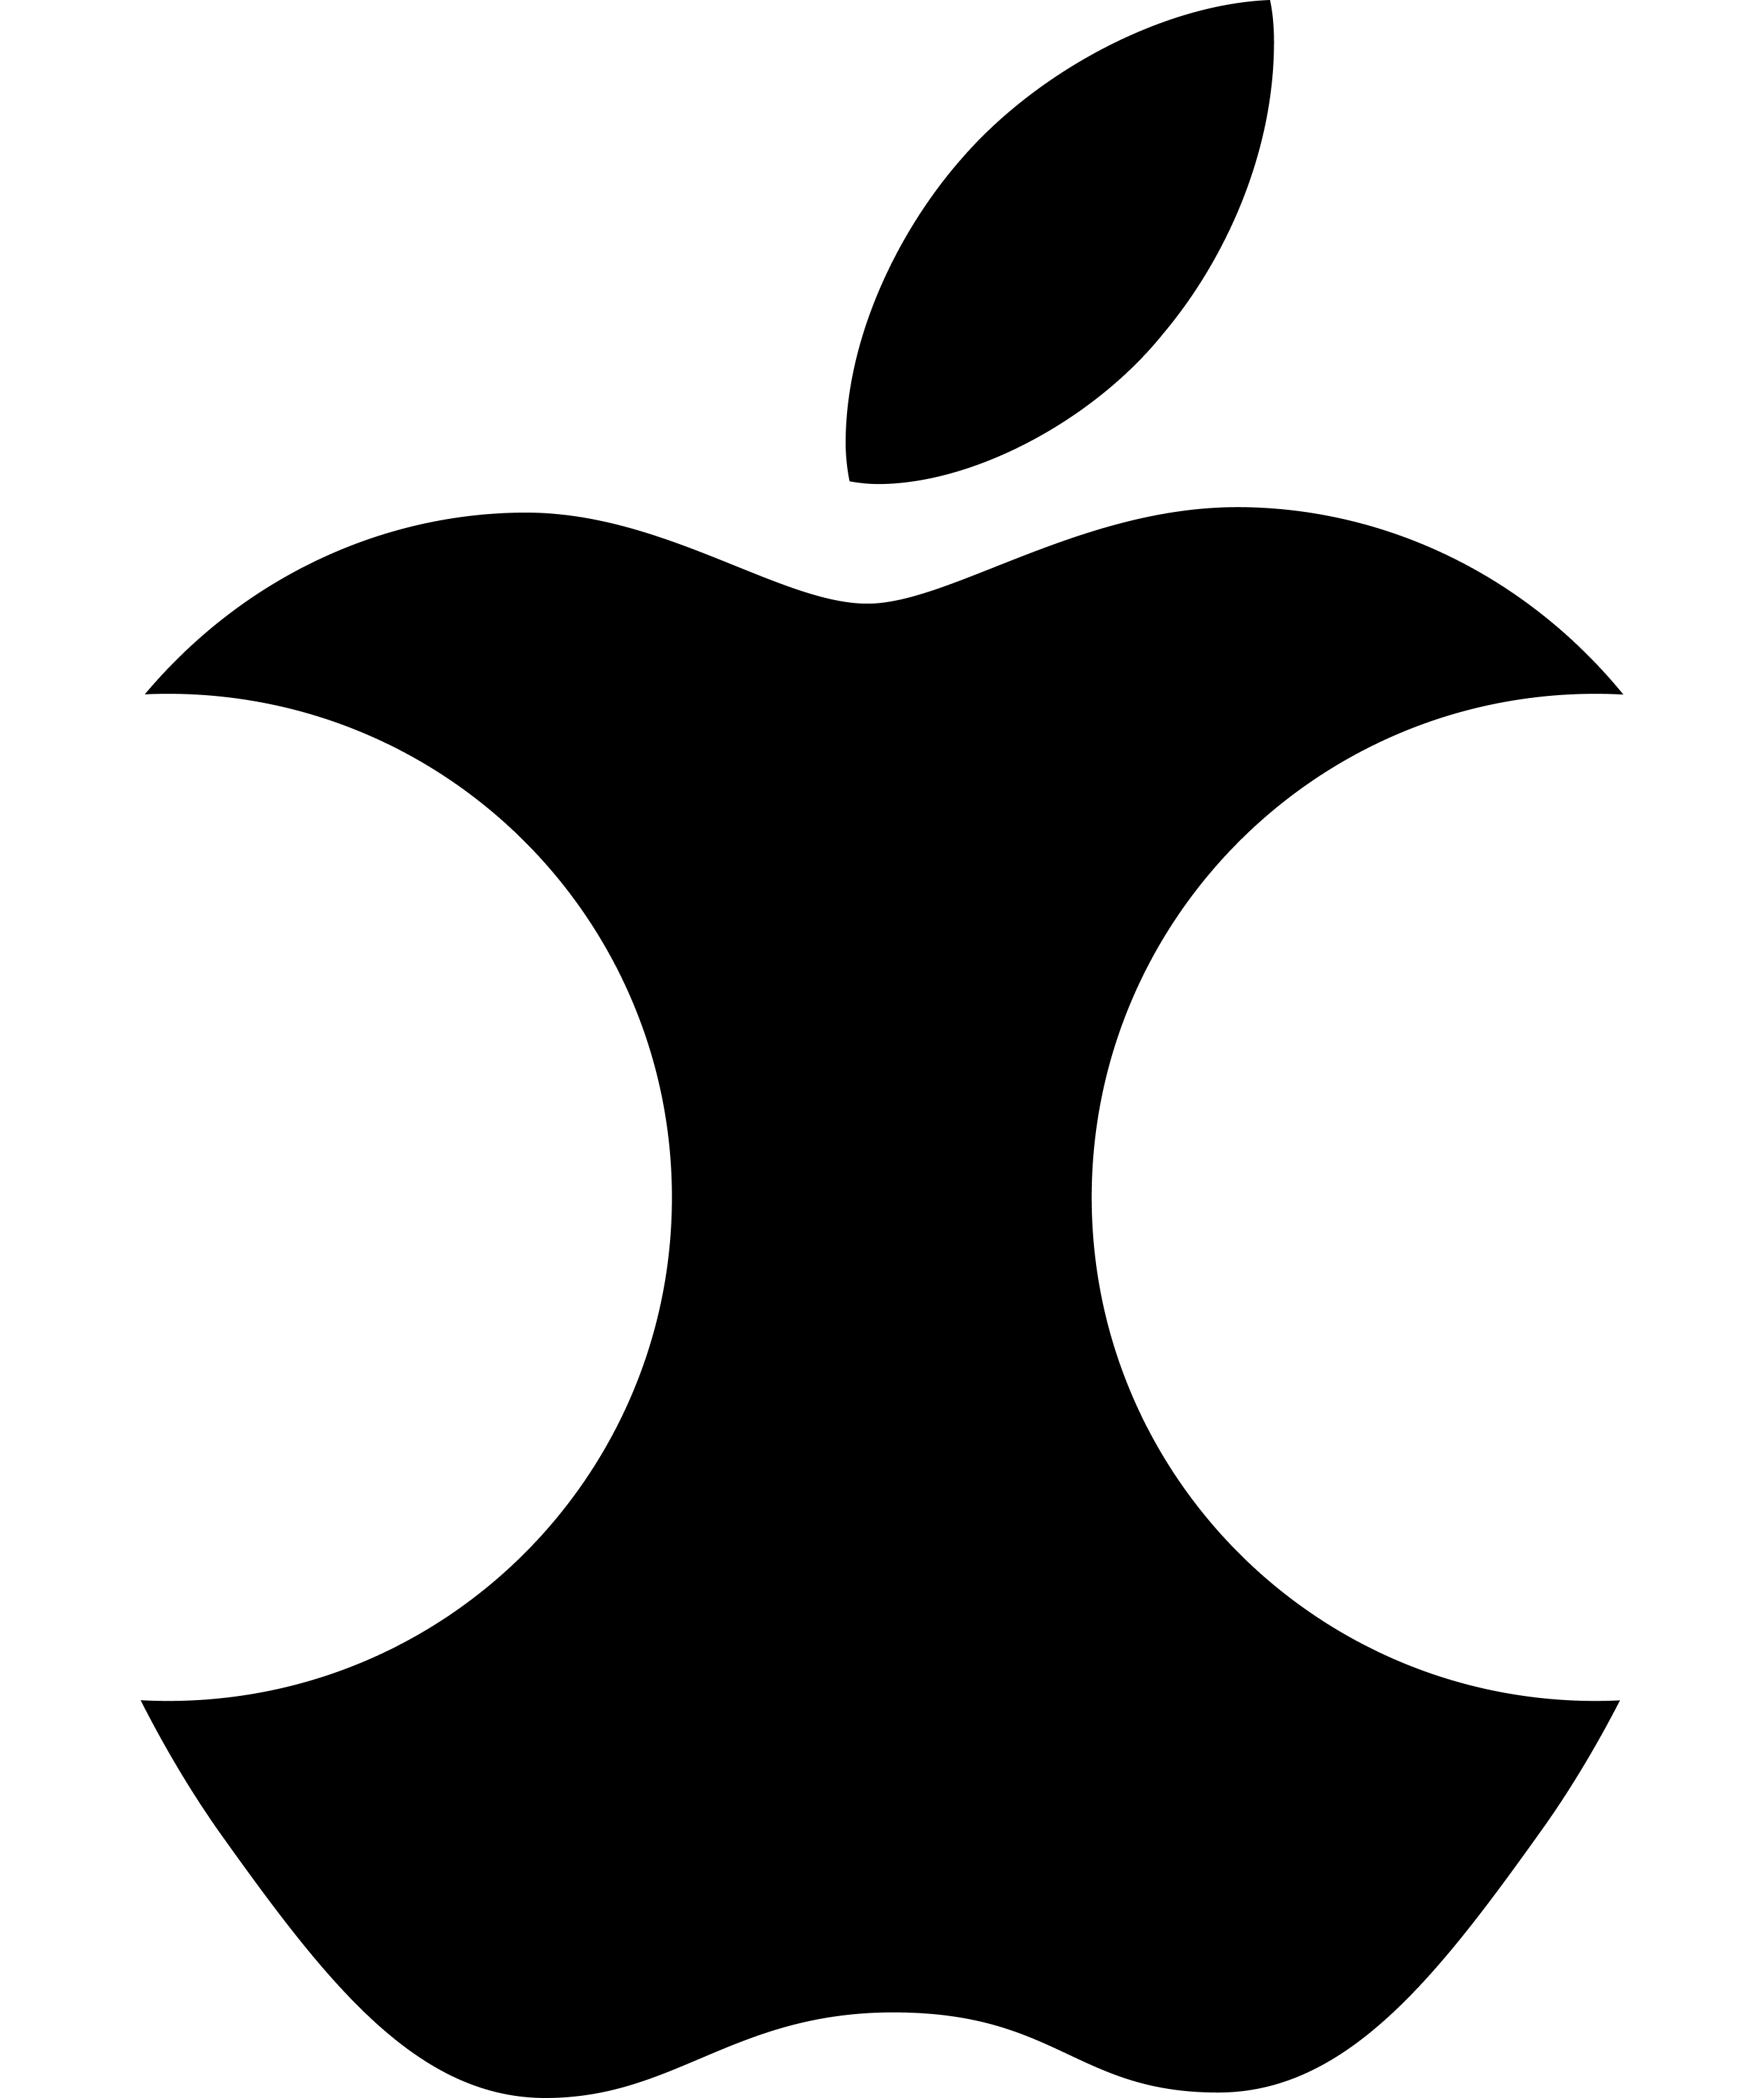
\includegraphics[width=0.25\textwidth]{./resources/empty_apple.png}

    \pause[]

    \vphantom{}

    \Large{\(\color{red}{abc} \color{black}{\cdot d \cdot} \color{red}{cba}\)}
  \end{block}
\end{frame}

\begin{frame}{\myframetitle}
  \begin{block}{Le trognon d'un mot}
    \centering
    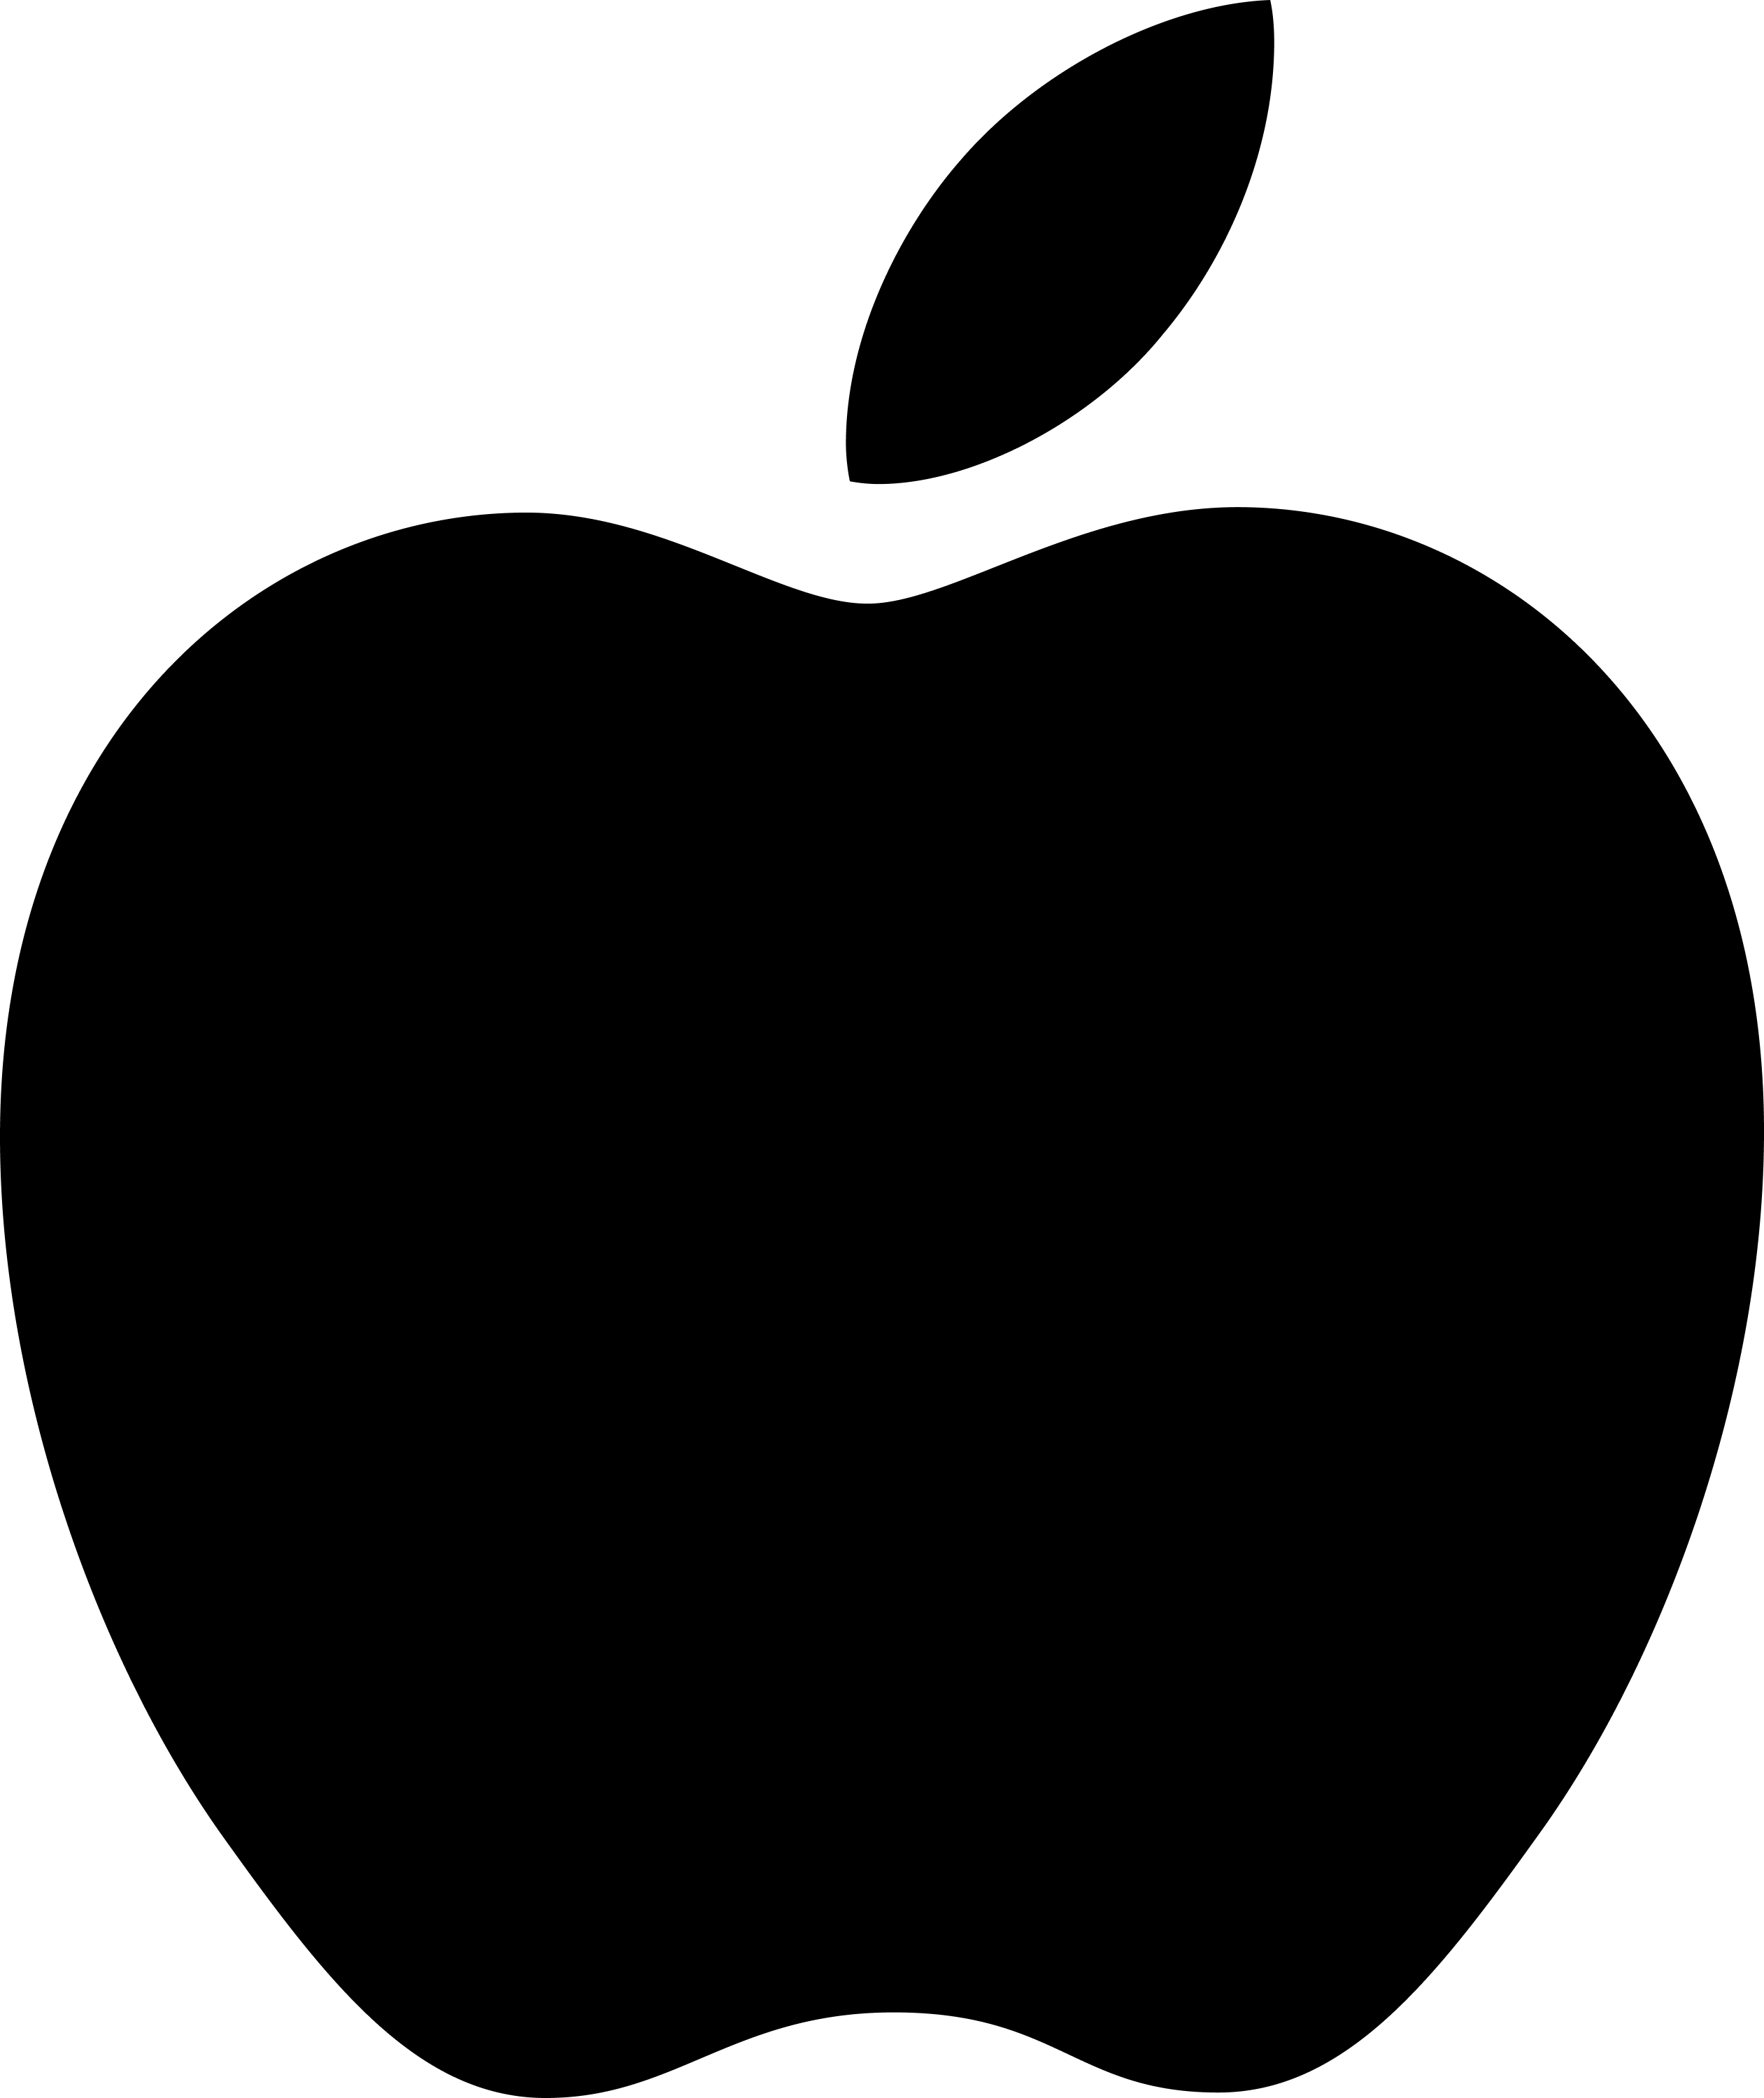
\includegraphics[width=0.25\textwidth]{./resources/full_apple.png}

    \pause[]

    \vphantom{}

    \Large{\(\color{red}{\varepsilon} \color{black}{\cdot abcdcba \cdot}
    \color{red}{\varepsilon}\)}
  \end{block}
\end{frame}

\begin{frame}{\myframetitle}
  \begin{definition}[Le trognon d'un mot]
    Le trognon d'un langage sera alors l'union des trognons des mots qu'il le
    compose.
  \end{definition}
\end{frame}

\subsection{Algorithme de grignotage}

\setframetitle{Algorithme de grignotage}

\begin{frame}{\myframetitle}
  \begin{example}[\(L(M) = a \cdot a^* \cdot c \cdot a^* \cdot a\)]
    \begin{center}
      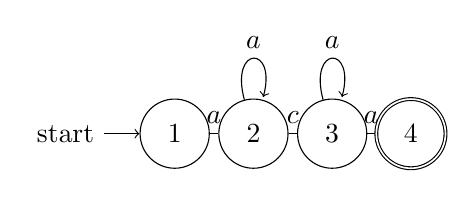
\begin{tikzpicture}
        \node[state, initial] (1) {\(1\)};
        \node[state, right of=1] (2) {\(2\)};
        \node[state, right of=2] (3) {\(3\)};
        \node[state, accepting, right of=3] (4) {\(4\)};

        \draw
        (1) edge[above] node{\(a\)} (2)
        (2) edge[loop above] node{\(a\)} (2)
        (2) edge[above] node{\(c\)} (3)
        (3) edge[loop above] node{\(a\)} (3)
        (3) edge[above] node{\(a\)} (4);
      \end{tikzpicture}
    \end{center}
  \end{example}
\end{frame}

\begin{frame}{\myframetitle}
  \begin{example}[\(M\) grignoté de \(a\)]
    \begin{center}
      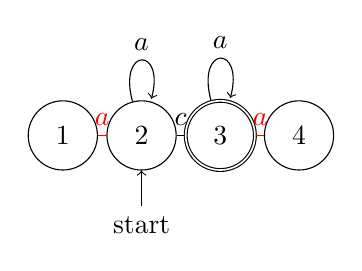
\begin{tikzpicture}
        \node[state] (1) {\(1\)};
        \node[state, initial below, right of=1] (2) {\(2\)};
        \node[state, accepting, right of=2] (3) {\(3\)};
        \node[state, right of=3] (4) {\(4\)};

        \draw
        (1) edge[above, red] node{\(a\)} (2)
        (2) edge[loop above] node{\(a\)} (2)
        (2) edge[above] node{\(c\)} (3)
        (3) edge[loop above] node{\(a\)} (3)
        (3) edge[above, red] node{\(a\)} (4);
      \end{tikzpicture}
    \end{center}
  \end{example}
\end{frame}

\begin{frame}{\myframetitle}
  \begin{example}[\(M\) grignoté de \(aa\)]
    \begin{center}
      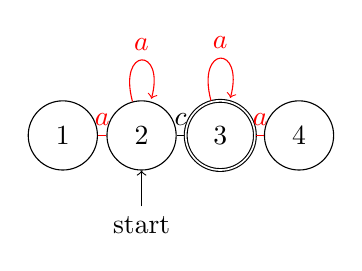
\begin{tikzpicture}
        \node[state] (1) {\(1\)};
        \node[state, initial below, right of=1] (2) {\(2\)};
        \node[state, accepting, right of=2] (3) {\(3\)};
        \node[state, right of=3] (4) {\(4\)};

        \draw
        (1) edge[above, red] node{\(a\)} (2)
        (2) edge[loop above, red] node{\(a\)} (2)
        (2) edge[above] node{\(c\)} (3)
        (3) edge[loop above, red] node{\(a\)} (3)
        (3) edge[above, red] node{\(a\)} (4);
      \end{tikzpicture}
    \end{center}
  \end{example}
\end{frame}

\begin{frame}{\myframetitle}
  \begin{definition}
    L'automate \(\texttt{nibbling}(M)\) sera donc l'union des automates
    grignotés distincts.
  \end{definition}

  \pause[]

  \begin{block}{Compléxité en état de notre algorithme}
    Le nombre d'états de l'union de deux automates est égal à la somme des
    nombres d'états des automates.

    \pause[]

    \vphantom{}

    Les automates grignotés ont comme forme \((Q, I, F, \delta)\) avec \(Q\)
    et \(\delta\) les mêmes et comme changement \(I\) et \(F\) qui sont deux
    ensembles non vides.

    \pause[]

    \vphantom{}

    Ce qui nous donne comme complexité finale~: \(n(2^n - 1)^2\) états.
  \end{block}
\end{frame}


\section{Langage permuté}

\subsection{Définition}

\setframetitle{Définition}

\begin{frame}{\myframetitle}
  \begin{definition}[\(Twist(L)\)]
    Le langage \(Twist(L)\) sera défini comment l'ensemble des mots du
    langage de \(L\) tel qu'on aura échangé les lettres aux indices \(2k\) et
    \(2k + 1\) avec \(k\in \mathbb{N}\).
  \end{definition}

  \pause[]

  \begin{example}
    \vspace*{-\baselineskip}
    \begin{align*}
      L &= \{\varepsilon, a, ab, abcd\} \\
      Twist(L) &= \{\varepsilon, a, ba, badc\}
    \end{align*}
  \end{example}
\end{frame}

\subsection{Algorithme twister}

\setframetitle{Algorithme twister}

\begin{frame}{\myframetitle}
  \begin{example}[Soit l'automate \(M\) suivant]
    \centering
    \begin{tikzpicture}
      \tikzset{
        ->,
        >=stealth',
        node distance=2.5cm,
        every state/.style={thick},
        initial text=$ $,
      }
      \node[state, initial] (q1) {\(1\)};
      \node[state, right of=q1] (q2) {\(2\)};
      \node[state, accepting, right of=q2] (q3) {\(3\)};
      \node[state, above right of=q3] (q4) {\(4\)};
      \node[state, right of=q4] (q5) {\(5\)};
      \node[state, accepting, right of=q5] (q6) {\(6\)};
      \node[state, right of=q3] (q7) {\(7\)};
      \node[state, accepting, right of=q7] (q8) {\(8\)};
      \node[state, right of=q8] (q9) {\(9\)};
      \node[state, accepting, below right of=q3] (q10) {\(10\)};
      \node[state, right of=q10] (q11) {\(11\)};
      \node[state, right of=q11] (q12) {\(12\)};

      \only<1> {
        \draw
          (q1) edge[above] node[blue]{\(b\)} (q2)
          (q2) edge[above] node[red]{\(a\)} (q3)
          (q3) edge[above] node[blue]{\(b\)} (q4)
          (q4) edge[above] node[red]{\(a\)} (q5)
          (q5) edge[above] node[blue]{\(b\)} (q6)
          (q3) edge[above] node[blue]{\(a\)} (q7)
          (q7) edge[above] node[red]{\(b\)} (q8)
          (q8) edge[above] node[blue]{\(b\)} (q9)
          (q3) edge[above] node[blue]{\(b\)} (q10)
          (q10) edge[above] node[red]{\(b\)} (q11)
          (q11) edge[above] node[blue]{\(a\)} (q12);
      }
      \only<2> {
        \draw
          (q1) edge[above] node[red]{\(a\)} (q2)
          (q2) edge[above] node[blue]{\(b\)} (q3)
          (q3) edge[above] node[red]{\(a\)} (q4)
          (q4) edge[above] node[blue]{\(b\)} (q5)
          (q5) edge[above] node[blue]{\(b\)} (q6)
          (q3) edge[above] node[red]{\(b\)} (q7)
          (q7) edge[above] node[blue]{\(a\)} (q8)
          (q8) edge[above] node[blue]{\(b\)} (q9)
          (q3) edge[above] node[red]{\(b\)} (q10)
          (q10) edge[above] node[blue]{\(b\)} (q11)
          (q11) edge[above] node[blue]{\(a\)} (q12);
      }
    \end{tikzpicture}
  \end{example}
\end{frame}

\begin{frame}{\myframetitle}
  \begin{example}[Soit l'automate \(N\) suivant]
    \centering
    \only<1-2> {
      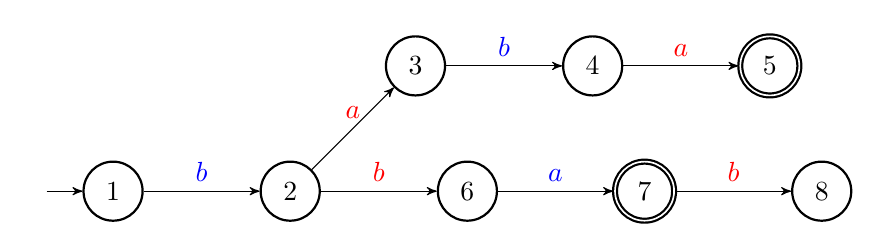
\begin{tikzpicture}
        \tikzset{
          ->,
          >=stealth',
          node distance=2.25cm,
          every state/.style={
            thick,
            inner sep = 0pt,
            minimum size = 0.75cm,
          },
          initial text=$ $,
        }
        \node[state, initial] (q1) {\(1\)};
        \node[state, right of=q1] (q2) {\(2\)};
        \node[state, above right of=q2] (q3) {\(3\)};
        \node[state, right of=q3] (q4) {\(4\)};
        \node[state, accepting, right of=q4] (q5) {\(5\)};
        \node[state, right of=q2] (q6) {\(6\)};
        \node[state, accepting, right of=q6] (q7) {\(7\)};
        \node[state, right of=q7] (q8) {\(8\)};

        \draw
          (q1) edge[above] node[blue]{\(b\)} (q2)
          (q2) edge[above] node[red]{\(a\)} (q3)
          (q3) edge[above] node[blue]{\(b\)} (q4)
          (q4) edge[above] node[red]{\(a\)} (q5)
          (q2) edge[above] node[red]{\(b\)} (q6)
          (q6) edge[above] node[blue]{\(a\)} (q7)
          (q7) edge[above] node[red]{\(b\)} (q8);
      \end{tikzpicture}

      \pause[]

      \vphantom{}

      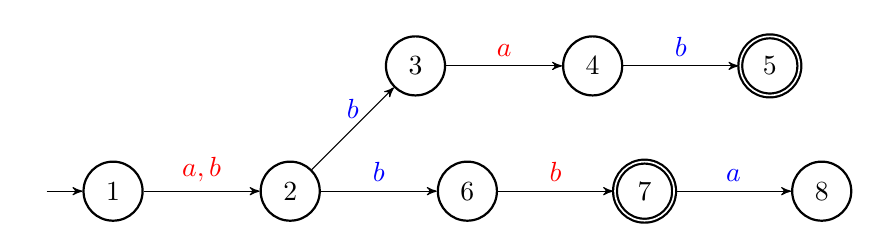
\begin{tikzpicture}
        \tikzset{
          ->,
          >=stealth',
          node distance=2.25cm,
          every state/.style={
            thick,
            inner sep = 0pt,
            minimum size = 0.75cm,
          },
          initial text=$ $,
        }
        \node[state, initial] (q1) {\(1\)};
        \node[state, right of=q1] (q2) {\(2\)};
        \node[state, above right of=q2] (q3) {\(3\)};
        \node[state, right of=q3] (q4) {\(4\)};
        \node[state, accepting, right of=q4] (q5) {\(5\)};
        \node[state, right of=q2] (q6) {\(6\)};
        \node[state, accepting, right of=q6] (q7) {\(7\)};
        \node[state, right of=q7] (q8) {\(8\)};

        \draw
          (q1) edge[above] node[red]{\(a, b\)} (q2)
          (q2) edge[above] node[blue]{\(b\)} (q3)
          (q3) edge[above] node[red]{\(a\)} (q4)
          (q4) edge[above] node[blue]{\(b\)} (q5)
          (q2) edge[above] node[blue]{\(b\)} (q6)
          (q6) edge[above] node[red]{\(b\)} (q7)
          (q7) edge[above] node[blue]{\(a\)} (q8);
      \end{tikzpicture}
    }
    \only<3-4> {
      \begin{tikzpicture}
        \tikzset{
          ->,
          >=stealth',
          node distance=2.25cm,
          every state/.style={
            thick,
            inner sep = 0pt,
            minimum size = 0.75cm,
          },
          initial text=$ $,
        }
        \node[state, initial] (q1) {\(1\)};
        \node[state, right of=q1] (q2b) {\(2_b\)};
        \node[state, left of=q3] (q2a) {\(2_a\)};
        \node[state, above right of=q2b] (q3) {\(3\)};
        \node[state, right of=q3] (q4) {\(4\)};
        \node[state, accepting, right of=q4] (q5) {\(5\)};
        \node[state, right of=q2] (q6) {\(6\)};
        \node[state, accepting, right of=q6] (q7) {\(7\)};
        \node[state, right of=q7] (q8) {\(8\)};

        \draw
          (q1) edge[above] node[blue]{\(b\)} (q2a)
          (q1) edge[above] node[blue]{\(b\)} (q2b)
          (q2a) edge[above] node[red]{\(a\)} (q3)
          (q3) edge[above] node[blue]{\(b\)} (q4)
          (q4) edge[above] node[red]{\(a\)} (q5)
          (q2b) edge[above] node[red]{\(b\)} (q6)
          (q6) edge[above] node[blue]{\(a\)} (q7)
          (q7) edge[above] node[red]{\(b\)} (q8);
      \end{tikzpicture}

      \pause[4]

      \vphantom{}

      \begin{tikzpicture}
        \tikzset{
          ->,
          >=stealth',
          node distance=2.25cm,
          every state/.style={
            thick,
            inner sep = 0pt,
            minimum size = 0.75cm,
          },
          initial text=$ $,
        }
        \node[state, initial] (q1) {\(1\)};
        \node[state, right of=q1] (q2b) {\(2_b\)};
        \node[state, left of=q3] (q2a) {\(2_a\)};
        \node[state, above right of=q2b] (q3) {\(3\)};
        \node[state, right of=q3] (q4) {\(4\)};
        \node[state, accepting, right of=q4] (q5) {\(5\)};
        \node[state, right of=q2] (q6) {\(6\)};
        \node[state, accepting, right of=q6] (q7) {\(7\)};
        \node[state, right of=q7] (q8) {\(8\)};

        \draw
          (q1) edge[above] node[red]{\(a\)} (q2a)
          (q1) edge[above] node[red]{\(b\)} (q2b)
          (q2a) edge[above] node[blue]{\(b\)} (q3)
          (q3) edge[above] node[red]{\(a\)} (q4)
          (q4) edge[above] node[blue]{\(b\)} (q5)
          (q2b) edge[above] node[blue]{\(b\)} (q6)
          (q6) edge[above] node[red]{\(b\)} (q7)
          (q7) edge[above] node[blue]{\(a\)} (q8);
      \end{tikzpicture}
    }
  \end{example}
\end{frame}

\begin{frame}{\myframetitle}
  \begin{block}{Automate quelconque}
    Si on ajoute les cycles, on devra alors supposer que tous n\oe{}uds
    intermédiaire se trouve dans le cas du n\oe{}ud \(2\), on devra donc le
    dupliquer.
  \end{block}
\end{frame}

\begin{frame}{\myframetitle}
  \begin{example}
    \centering
    \only<1-2> {
      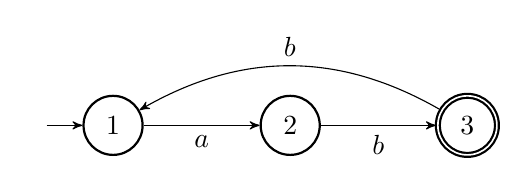
\begin{tikzpicture}
        \tikzset{
          ->,
          >=stealth',
          node distance=2.25cm,
          every state/.style={
            thick,
            inner sep = 0pt,
            minimum size = 0.75cm,
          },
          initial text=$ $,
        }
        \node[state, initial] (1) {\(1\)};
        \node[state, right of=1] (2) {\(2\)};
        \node[state, accepting, right of=2] (3) {\(3\)};
        \draw
          (1) edge[below] node{\(a\)} (2)
          (2) edge[below] node{\(b\)} (3)
          (3) edge[bend right, above] node{\(b\)} (1);
      \end{tikzpicture}
    }
    \only<2> {
      \begin{tikzpicture}
        \tikzset{
          ->,
          >=stealth',
          node distance=2.25cm,
          every state/.style={
            thick,
            inner sep = 0pt,
            minimum size = 0.75cm,
          },
          initial text=$ $,
        }
        \node[state, initial] (1) {\(1\)};
        \node[state, above of=3] (1a) {\(1_a\)};
        \node[state, right of=1] (2b) {\(2_b\)};
        \node[state, above of=2b] (2) {\(2\)};
        \node[state, accepting, right of=2b] (3) {\(3\)};
        \node[state, accepting, above of=1] (3b) {\(3_b\)};
        \draw
          (1) edge[below] node{\(b\)} (2b)
          (2b) edge[below] node{\(a\)} (3)
          (3) edge[right] node{\(a\)} (1a)
          (1a) edge[above] node{\(b\)} (2)
          (2) edge[above] node{\(b\)} (3b)
          (3b) edge[left] node{\(b\)} (1);
      \end{tikzpicture}
    }
  \end{example}
\end{frame}

\begin{frame}{\myframetitle}
  \begin{block}{Compléxité en état de notre algorithme}
    Dans le pire cas, notre algorithme dupliquera tous les états de
    l'automate. 

    \pause[]
    \vphantom{}

    Sachant que chaque état peut être dupliqué étant de voir qu'il y a de
    symbole de l'alphabet plus un. 

    \pause[]
    \vphantom{}

    Alors, la complexité dans le pire cas de notre algorithme est \(n(\lvert
    \Sigma \rvert + 1)\).
  \end{block}
\end{frame}

% !chktex-file 8
% !chktex-file 41

\section{Conclusion}

\setframetitle{Conclusion}

\begin{frame}{\myframetitle}
  \begin{block}{Conclusion}
    On a donc que pour un alphabet binaire~:
    \begin{itemize}
      \item la concaténation de deux langages a une complexité de
        \(m2^n - 2^{n - 1}\),
      \item le renverser (à un état initial) d'un langage à une complexité de
        \((n + 1)\),
    \end{itemize}
  \end{block}
\end{frame}

\begin{frame}{\myframetitle}
  \begin{block}{Ouverture}
    On pourrait s'intéresser aux opérations~:
    \begin{itemize}
      \item<2-> celle de permutation (\textit{Twist}),
      \item<3-> celle de grignotage (\textit{Trognon}).
    \end{itemize}
  \end{block}
\end{frame}

\printbibliography

\end{document}
